\documentclass[conference]{IEEEtran}
\def\BibTeX{{\rm B\kern-.05em{\sc i\kern-.025em b}\kern-.08em
    T\kern-.1667em\lower.7ex\hbox{E}\kern-.125emX}}
\usepackage{amsmath,amssymb,amsfonts}
\usepackage{algorithmic}
\usepackage{graphicx}
\usepackage{textcomp}
\usepackage{xcolor}
\usepackage{xspace}
\usepackage[numbers,sort&compress]{natbib}
\usepackage{stmaryrd}
\usepackage{listings}
\usepackage{verbatim}
\usepackage{xcolor}  % for setting colors
\usepackage{url}
\usepackage{float}
\usepackage{multirow}
\usepackage{colortbl}
% \usepackage{showlabels}
\usepackage{amsthm}
\usepackage{tikz}

%counters
\newcounter{stddefctr}
\setcounter{stddefctr}{1}
\newcounter{extdefctr}
\setcounter{extdefctr}{1}

% Define Python style for listings
\lstdefinestyle{pythonstyle}{
    language=Python,
    basicstyle=\ttfamily\small,
    keywordstyle=\color{blue},
    commentstyle=\color{green},
    stringstyle=\color{red},
    frame=none,
    breaklines=true,
    morekeywords={yield}
}

% Edit the mod command to take less space
\let\oldmod\mod
\renewcommand{\mod}[1]{\hspace{-7pt} \oldmod \, #1}

% Define the note command
\newcommand{\note}[1]{\small\textcolor{purple}{#1}\normalsize}

% Define a concat command
\newcommand*\concat{\mathbin{\|}}

% Define a macro for the floor function
\newcommand{\floor}[1]{\left\lfloor #1 \right\rfloor}

% Define a macro for the ceiling function
\newcommand{\ceil}[1]{\left\lceil #1 \right\rceil}

% Define a macro for a tuple using angled brackets
\newcommand{\tuple}[1]{\langle #1 \rangle}

% Shorthands
\newcommand{\TMS}{Thue-Morse Sequence\xspace}
\newcommand{\ETMS}{Extended Thue-Morse Sequence\xspace}
\newcommand{\Integers}{\mathbb{Z}}
\newcommand{\Naturals}{\mathbb{N}}
\newcommand{\totaloriginals}{15}
\newcommand{\totalextensions}{9}
\newcommand{\TotalOriginals}{\totaloriginals\xspace}
\newcommand{\TotalExtensions}{\totalextensions\xspace}
\newcommand{\TotalDefs}{\the\numexpr \totaloriginals + \totalextensions \relax\xspace}


\begin{document}

\title{Extending The \TMS}

\author{\IEEEauthorblockN{Olivia Appleton-Crocker}
\IEEEauthorblockA{\textit{TMW Center for Early Learning + Public Health}\\
\textit{University of Chicago}\\
Chicago, Illinois, United States\\
ORCID: 0009-0004-2296-7033}}

\maketitle
\thispagestyle{plain}
\pagestyle{plain}

\begin{abstract}
In this paper, we discuss various ways to extend the \TMS \cite{OEIS-TMS} when used as a fair-share sequence. Included are \TotalOriginals definitions of the original sequence, \TotalExtensions extensions to n players, for a total of \TotalDefs definitions. Also included are proofs of equality for all definitions, as well as an examination of several properties of the \TMS and their presence in the \ETMS. In the appendix are several complexity analyses for both time and space of each definition.
\end{abstract}

\begin{IEEEkeywords}
Combinatorics, Generating Functions, Thue-Morse, Prouhet-Thue-Morse, Formal Languages, Number Theory, Periodicity, Aperiodicity, Rotation, Concatenation
\end{IEEEkeywords}

\section{Introduction}

\note{This section is too fluffy. Probably needs to be rewritten entirely}

The \TMS is a fundamental object in combinatorics and theoretical computer science, widely studied for its remarkable properties and diverse applications. It is often presented as an infinite sequence starting with 0, as shown below: \begin{equation*}
T\!\!=\!\!\tuple{0,\!1,\!1,\!0,\!1,\!0,\!0,\!1,\!1,\!0,\!0,\!1,\!0,\!1,\!1,\!0,\!1,\!0,\!0,\!1,\!0,\!1,\!1,\!0,\!0,\!1,\!1,\!0,\!\ldots}
\end{equation*}

This sequence arises in various fields, including automata theory, formal languages, number theory, and signal processing, due to its connection to binary operations, periodicity, and complexity. Its structure has been examined in relation to notions of minimality and non-repetitiveness, making it a natural object of study in mathematical logic and computational theory.

Over the past two centuries, the \TMS has garnered attention for its role in constructing infinite words with specific properties (such as non-repetition over large substrings) and for its use in the design of error-correcting codes, pseudorandom number generators, and tiling problems. More recently, its applications have extended to the analysis of dynamical systems, coding theory, and the study of complexity within algorithms.

This survey primarily aims to explore the various definitions of the \TMS found in the literature, with an emphasis on identifying distinct formulations and categorizing them. Additionally, this work seeks to extend these definitions from the binary alphabet $\{0,1\}$ to larger alphabets $\{0,1,\dots,n\!\!-\!\!1\}$, often referred to as ``integer bases.'' This work aims to explore how properties such as non-repetition, periodicity, and complexity are preserved under these extensions. By systematically analyzing these extensions and their associated properties, this overview hopes to present a deeper understanding of the \TMS's generalizations and their potential applications in broader contexts.

This paper is divided into 8 sections. In Section 1, we introduce the concepts built upon in this paper. In Section 2 we present each of the \TotalOriginals definitions of the standard \TMS as seen in the literature today, divided by category of definition. We first look at numeric methods, then operations on ordered collections of numbers. We next examine definitions that relate to other sequences of integers, followed by a pair of generating functions, a hypergeometric definition, one based on cellular automatons, and a derivation from Galois Duels.

In Section 3 we prove their equivalence with each other in the standard base-2 domain. In Section 4 we present \TotalExtensions definitions that extend into larger domains. Most of these can only construct sequences with integer value elements, though a select few can be extended into even broader domains, such as rational bases. In Section 5 we prove that the extensions are equivalent to each other in the domain of positive integer bases. In Section 6 we examine the preservation (or failure) of properties for the standard \TMS when extended to larger bases. Sections 7 and 8 are acknowledgments and the appendix respectively. The appendix contains honorable mention extensions and complexity analyses (both time and space) for the different definitions. These show which may be the most computationally efficient ways to calculate the \TMS or \ETMS, given your available resources.

\section{The Original Sequence}

\subsection{Definition \arabic{stddefctr} of \TotalOriginals\xspace --- Parity of Hamming Weight}

This definition appears in \cite{Spiegelhofer_2020, Allouche-Shallit_1999, pannipitiya_2024, OEIS-TMS}.

The Hamming Weight, as typically defined, is the digit sum of a binary number. In other words, it is a count of the high bits in a given number. A common way to generate the \TMS is to take the parity\footnote{Whether a number is odd or even} of the Hamming Weight\footnote{The count of $1$s in the binary representation of a number} for each natural number. We can define that as follows:

\begin{equation}
    \edef\tempLabel{eq:p2_d\arabic{stddefctr}}
    \label{\tempLabel}
    \begin{aligned}
      p(0) &= 0 \\
      p(n) &= (n \; \mod{2}) + p\left(\floor{\dfrac{n}{2}}\right) \\
T_{2,\arabic{stddefctr}}(n) &= p(n) \; \mod{2}
    \end{aligned}
\end{equation}

The subscript indicates that we are using $2$ players (writing in base $2$) and that we are using the first definition laid out in this paper. Note that when we extend to n players, the $T$ function will get a second parameter for the number of players, so it will look like $T_{n,d}(x, s)$, where $s$ is the size of the player pool, and therefore the base we use to define the sequence.

\stepcounter{stddefctr}
\subsection{Definition \arabic{stddefctr} of \TotalOriginals\xspace --- Powers of Negative One}

This appears in \cite{OEIS-TMS-inv}.

Another way to implement the modularity of the previous definition is to use the appropriate root of unity. In this paper, we use $\omega_s = \exp\left(\tfrac{2i\pi}{s}\right)$ to represent the primitive root of unity in base $s$, such that $(\omega_s)^s = 1$. Because of this, extracting the power of $(\omega_s)^x$ will give you the same value as $x \; \mod{s}$.

There are two ways this can be approached. In the first we work with these output values directly, mapping $\{1, -1\} \to \{0, 1\}$:

\begin{equation}
    \edef\tempLabel{eq:p2_d\arabic{stddefctr}}
    \label{\tempLabel}
    \begin{aligned}
T_{2,\arabic{stddefctr}a}(n) &= \dfrac{1 - (\omega_2)^{p(n)}}{2} \\
                             &= \dfrac{1 - (-1)^{p(n)}}{2}
    \end{aligned}
\end{equation}

\stepcounter{stddefctr}
\subsection{Definition \arabic{stddefctr} of \TotalOriginals\xspace --- Root of Unity}

And in the second we extract the exponent:

\begin{equation}
    \edef\tempLabel{eq:p2_d\arabic{stddefctr}b}
    \label{\tempLabel}
    \begin{aligned}
T_{2,\arabic{stddefctr}b}(n) &= \dfrac{\log\left(\omega_2^{p(n)}\right)}{\log\left(\omega_2\right)} \\
                             &= \dfrac{\log\left((-1)^{p(n)}\right)}{\log(-1)} \\
                             &= \dfrac{(p(n) \mod{2}) \cdot \log(-1)}{\log(-1)} \\
                             &= \dfrac{(p(n) \mod{2}) \cdot i\pi}{i\pi} \\
                             &= p(n) \mod{2}
    \end{aligned}
\end{equation}

\stepcounter{stddefctr}
\subsection{Definition \arabic{stddefctr} of \TotalOriginals\xspace --- Recursion}

This definition appears in \cite{Kolář-Nori_1991, pannipitiya_2024, OEIS-TMS}.

\begin{equation}
    \edef\tempLabel{eq:p2_d\arabic{stddefctr}}
    \label{\tempLabel}
    \begin{aligned}
   T_{2,\arabic{stddefctr}}(0) &= 0 \\
  T_{2,\arabic{stddefctr}}(2n) &= T_{2,\arabic{stddefctr}}(n) \\
T_{2,\arabic{stddefctr}}(2n+1) &= 1 - T_{2,\arabic{stddefctr}}(n)
    \end{aligned}
\end{equation}

\stepcounter{stddefctr}
\subsection{Definition \arabic{stddefctr} of \TotalOriginals\xspace --- Floor-Ceiling Difference}

This definition appears in \cite{OEIS-TMS}. \note{Some of the info that's in the proof of equivalence should be lifted up into here}

\begin{equation}
    \edef\tempLabel{eq:p2_d\arabic{stddefctr}}
    \label{\tempLabel}
    \begin{aligned}
      b(n) &= \begin{cases}
          n &\text{if } n \le 1 \\
          b\left(\ceil{\dfrac{n}{2}}\right) - b\left(\floor{\dfrac{n}{2}}\right) &\text{otherwise}
\end{cases} \\
T_{2,\arabic{stddefctr}}(n-1) &= \dfrac{1 - b(2n - 1)}{2} \pmod{2}
    \end{aligned}
\end{equation}

\note{This seems very similar to the highest bit difference definition, and I think it may be what that was derived from}

\stepcounter{stddefctr}
\subsection{Definition \arabic{stddefctr} of \TotalOriginals\xspace --- Highest Bit Difference}

This definition appears in \cite{Arndt_2010}.

\note{The text below is from Wiki and needs to be entirely rewritten. I was able to derive the formula on my own from translating their code. This method leads to a fast method for computing the \TMS: start with t0 = 0, and then, for each n, find the highest-order bit in the binary representation of n that is different from the same bit in the representation of n - 1. If this bit is at an even index, tn differs from tn - 1, and otherwise it is the same as tn - 1.}

\noindent\begin{minipage}[H]{0.48\textwidth}\begin{lstlisting}[style=pythonstyle]
from itertools import count

def p2_d07():
    value = 1
    for n in count():
        # Assumes that (-1).bit_length() == 1
        x = (n ^ (n - 1)).bit_length() + 1
        if x & 1 == 0:
            # Bit index even, so toggle value
            value = 1 - value
        yield value
\end{lstlisting}\end{minipage}

\note{Should there be a +1 inside that call to log2?}

\begin{equation}
    \edef\tempLabel{eq:p2_d\arabic{stddefctr}}
    \label{\tempLabel}
    \begin{aligned}
T_{2,\arabic{stddefctr}}(0) &= 0 \\
T_{2,\arabic{stddefctr}}(n) &= \begin{aligned}[c]
    &\floor{\log_2(n \oplus (n - 1))} \\
    &+ T_{2,\arabic{stddefctr}}(n - 1) \pm 1
\end{aligned} \pmod{2}
    \end{aligned}
\end{equation}

\stepcounter{stddefctr}
\subsection{Definition \arabic{stddefctr} of \TotalOriginals\xspace --- Hamming-Weight Complement}

This definition appears in \cite{OEIS-TMS-inv}. The Hamming Weight Complement (defined as $\overline{p}(n)$) is the count of $0$s in the minimal binary representation of a number, and A054429 is the sequence defined by reversing the order of integers between $2^n$ and $2^{n+1}-1$ (ex: $0, 1, 3, 2, 7, 6, 5, 4, \dots$).

\begin{equation}
\begin{aligned}
    \text{A054429}(n) &= \begin{cases}
        0 &\text{if } n = 0 \\
        3 \cdot 2^{\floor{\log_2(n)}} - n - 1 &\text{otherwise}
    \end{cases} \\
    \overline{p}(x) &= \ceil{\log_2(x + 1)} - p(x) \\
    T_{2,\arabic{stddefctr}}(n) &= 1 - \overline{p}(\text{A054429}(n)) \;\mod{2}
\end{aligned}
\end{equation}

\stepcounter{stddefctr}
\subsection{Definition \arabic{stddefctr} of \TotalOriginals\xspace --- Invert and Extend}

This definition appears in \cite{OEIS-TMS, Bolker_2016, pannipitiya_2024}.

This definition is more natural to think about as extending a tuple that contains the sequence. We will give a recurrence relation below, but to build an intuition we will work in this framework first.

Let $t(n)$ be the first $2^n$ elements of the \TMS. Given this, we can define\footnote{    
Using $\concat$ to mean concatenation, so $\tuple{0} \concat \tuple{1} = \tuple{0, 1}$. Likewise:

\;\;$\displaystyle\bigparallel_{i=a}^b f(i) = f(a) \concat f(a + 1) \concat f(a + 2) \concat \cdots \concat f(b)$
}:

\begin{equation}
\begin{aligned}
\text{inv}(\mathbf{x}) &= \begin{cases}
        0, &\text{if } x_i = 1 \\
        1, &\text{if } x_i = 0
    \end{cases} \\
    &\quad\quad\text{for } \mathbf{x} = \tuple{x_0, x_1, \ldots, x_{(|\mathbf{x}|-1)}} \\
                  t(0) &= \tuple{0} \\
                  t(n) &= t(n - 1) \concat \text{inv}(t(n - 1))
    \end{aligned}
\end{equation}

Given the above, we can define a recurrence relation that will give us individual elements. It will be less efficient to compute, but will allow proofs of equivalence to be easier.

\note{Should the below have a +1 inside the log?}

\begin{equation}
    \edef\tempLabel{eq:p2_d\arabic{stddefctr}}
    \label{\tempLabel}
    \begin{aligned}
T_{2,\arabic{stddefctr}}(0) &= 0 \\
T_{2,\arabic{stddefctr}}(n) &= T_{2,\arabic{stddefctr}}\left(n - 2^{\floor{\log_2(n)}}\right) + 1 \pmod{2}
    \end{aligned}
\end{equation}

\stepcounter{stddefctr}
\subsection{Definition \arabic{stddefctr} of \TotalOriginals\xspace --- Substitute and Flatten}

This definition appears in \cite{Spiegelhofer_2020, Kolář-Nori_1991, pannipitiya_2024, OEIS-TMS}. It is one of the most commonly used because of its simplicity. Define the morhpism $\mu$ on the alphabet $\{0, 1\}$ by $\mu(0) = 01, \mu(1) = 10$. $T$ is then the unique fixed point of $\mu$ that begins with $0$. In other words, $T = \lim_{n\to\infty}\mu^n(0)$.

\begin{equation}
    \edef\tempLabel{eq:p2_d\arabic{stddefctr}}
    \label{\tempLabel}
    \begin{aligned}
      s(n) &= \begin{cases}
          \tuple{0, 1}, &\text{if } n = 0 \\
          \tuple{1, 0}, &\text{if } n = 1
      \end{cases} \\
      t(0) &= \tuple{0} \\
      t(n) &= \bigparallel_{i=0}^{2^{n-1}-1} s(t(n-1)_i)  \\
T_{2,\arabic{stddefctr}}(n) &= t(\ceil{\log_2(n + 1)})_n
    \end{aligned}
\end{equation}

So for example, calculating $T_{2,\arabic{stddefctr}}(3)$ would look like:

\begin{equation}
    \begin{aligned}
      t(0) &= \tuple{0} \\
      t(1) &= \bigparallel_{i=0}^{0} s(t(0)_i) = \tuple{0, 1} \\
      t(2) &= \bigparallel_{i=0}^{1} s(t(1)_i) = \tuple{0, 1, 1, 0} \\
T_{2,\arabic{stddefctr}}(3) &= t(\ceil{\log_2(3 + 1)})_3 \\
           &= t(2)_3 \\
           &= \tuple{0, 1, 1, 0}_3 \\
           &= 0
    \end{aligned}
\end{equation}

\stepcounter{stddefctr}
\subsection{Definition \arabic{stddefctr} of \TotalOriginals\xspace --- Recursive Rotation}

Another way to phrase the above definition is as recursive rotation. To the best of our knowledge, this definition is original to this paper. If we decompose $s$, we can instead represent it as:

\begin{equation}
    \edef\tempLabel{eq:p2_d\arabic{stddefctr}}
    \label{\tempLabel}
    \begin{aligned}
r(\mathbf{x}, i) &= \begin{aligned}[c]
                   &\tuple{x_{0 + i \mod{|\mathbf{x}|}}, x_{1 + i \mod{|\mathbf{x}|}}, \ldots} \\
                   &\text{for } \mathbf{x} = \tuple{x_0, x_1, \ldots, x_{(|\mathbf{x}|-1)}}
        \end{aligned} \\
            t(0) &= \tuple{0} \\
            t(1) &= \tuple{0, 1} \\
            t(n) &= \bigparallel_{i=0}^1 r\left(t(n-1), i \cdot 2^{n-2}\right) \\
      T_{2,\arabic{stddefctr}}(n) &= t(\ceil{\log_2(n + 1)})_n
    \end{aligned}
\end{equation}

\stepcounter{stddefctr}
\subsection{Definition \arabic{stddefctr} of \TotalOriginals\xspace --- Odious Number Derivation}

This definition appears in \cite{OEIS-TMS}.

Another way to generate the \TMS is to take the sequence of Odious Numbers \cite{OEIS-Odious} mod $2$. Odious numbers are those with an odd number of $1$s in their binary representation. Note that the player numbers in this derivation are swapped, so when generating this for testing and extension, we add 1 to the result. Some simple generating code \cite{repo} for this is as follows:

\noindent\begin{minipage}[H]{0.48\textwidth}\begin{lstlisting}[style=pythonstyle]
from itertools import count

def seq_p2_d09():
    for i in count():
        if i.bit_count() & 1:
            yield (i + 1) & 1
\end{lstlisting}\end{minipage}

In mathematical terms, this can be translated to:

\begin{equation}
\edef\tempLabel{eq:p2_d\arabic{stddefctr}}
\label{\tempLabel}
\begin{aligned}
no(n) &= \begin{cases}
    n &\text{if } p(n) \mod{2} = 1 \\
    no(n+1) &\text{otherwise}
\end{cases} \\
o(n) &= \begin{cases}
    1              &\text{if }n = 0 \\
    no(o(n-1) + 1) &\text{if } n > 0
\end{cases} \\
T_{2,\arabic{stddefctr}}(n) &= o(n) + 1 \pmod{2}
\end{aligned}
\end{equation}

\note{Aren't Odious Numbers exactly the numbers where the parity of the hamming weight is 1? So doesn't that mean that the Thue-Morse Sequence selects which numbers are Odious? From cursory testing, it seems to. There's something to be had there.}

\note{A possible way to extend this would be to reinterpret this as where the digit sum is not n-even}

\note{A related definition on OEIS \cite{OEIS-TMS} is
\begin{equation*}
\begin{aligned}
    &T(n) + \text{Odious}(n - 1) + 1 = 2n \text{ for } n \ge 1 \\
    &T(n) = 2n - \text{Odious}(n - 1) - 1
\end{aligned}
\end{equation*}
}

\stepcounter{stddefctr}
\subsection{Definition \arabic{stddefctr} of \TotalOriginals\xspace --- Evil Numbers Derivation 1}

This definition appears in \cite{OEIS-TMS}. \note{More text}

The Evil Numbers \cite{OEIS-Evil} are those who have an even number of $1$s in their binary representation. Note that this is the opposite of the Odious Numbers referenced above.

\noindent\begin{minipage}[H]{0.48\textwidth}\begin{lstlisting}[style=pythonstyle]
from itertools import count

def evil():
    for i in count():
        if i.bit_count() & 1 == 0:
            yield i

def p2_d10():
    for n, i in enumerate(evil()):
        yield (i - 2 * n) & 1
\end{lstlisting}\end{minipage}

In mathematical terms, this can be translated to:

\begin{equation}
\edef\tempLabel{eq:p2_d\arabic{stddefctr}}
\label{\tempLabel}
\begin{aligned}
ne(n) &= \begin{cases}
    n &\text{if } p(n) \mod{2} = 1 \\
    ne(n+1) &\text{otherwise}
\end{cases} \\
e(n) &= \begin{cases}
    1              &\text{if }n = 0 \\
    ne(e(n-1) + 1) &\text{if } n > 0
\end{cases} \\
T_{2,\arabic{stddefctr}}(n) &= e(n) - 2n \pmod{2}
\end{aligned}
\end{equation}

\stepcounter{stddefctr}
\subsection{Definition \arabic{stddefctr} of \TotalOriginals\xspace --- Evil Numbers Derivation 2}

This definition ppears in \cite{OEIS-TMS-inv}. \note{More text}

A second, more-efficient derivation from the Evil Numbers is as follows, where $ce()$ is the count of Evil Numbers less than $n$ \cite{OEIS-A159481}, and $p()$ is the function defined in Equation \ref{eq:p2_d1}.

\begin{equation}
    \edef\tempLabel{eq:p2_d\arabic{stddefctr}}
    \label{\tempLabel}
    \begin{aligned}
     ce(n) &= \floor{\dfrac{n + 1}{2}} + p(n + 1) \cdot (n + 1 \mod{2}) \\
T_{2,\arabic{stddefctr}}(n) &= 1 - ce(n + 1) + ce(n)
    \end{aligned}
\end{equation}

\stepcounter{stddefctr}
\subsection{Definition \arabic{stddefctr} of \TotalOriginals\xspace --- Odious \& Evil Numbers Derivation}

This definition appears in \cite{OEIS-TMS-inv}. \note{More text as to why. Also, figure out why}

A second, more-efficient derivation from the Evil Numbers is as follows, where $ce()$ is the count of Evil Numbers less than $n$ \cite{OEIS-A159481}, and $p()$ is the function defined in Equation \ref{eq:p2_d1}.

\begin{equation}
    \edef\tempLabel{eq:p2_d\arabic{stddefctr}}
    \label{\tempLabel}
    \begin{aligned}
     oe(n) &= \begin{cases}
         o\left(\floor{\dfrac{n}{2}}\right) &\text{if } n \mod{2} = 0 \\
         e\left(\floor{\dfrac{n}{2}}\right) &\text{if } n \mod{2} = 1
     \end{cases} \\
T_{2,\arabic{stddefctr}}(n) &= 1 - oe(n) \pmod{2}
    \end{aligned}
\end{equation}

\stepcounter{stddefctr}
\subsection{Definition \arabic{stddefctr} of \TotalOriginals\xspace --- Gould's Sequence Derivation}

This definition appears in \cite{OEIS-TMS}.

Gould's Sequence \cite{OEIS-Gould} are the number of odd entries in a given row of Pascal's Triangle. Note that of the numeric methods, this is the least computationally efficient definition in this paper (see Tables \ref{tab:time_p2_d15} \& \ref{tab:space_p2_d15}).

\note{Why mod 3? Everything else is mod 2. This definition is unlikely to be extendable, and the obvious routes fail. I don't get why this works, and I think I need to. I \textit{think} $\text{Gould}(x)$ always returns $2k + \{0,1\}$}

\begin{equation}
    \edef\tempLabel{eq:p2_d\arabic{stddefctr}}
    \label{\tempLabel}
    \begin{aligned}
T_{2,\arabic{stddefctr}}(n) &= \text{Gould}(n) - 1 \mod{3} \\
            &= \left(\sum_{k=0}^n \left(\binom{n}{k} \mod{2} \right)\right) - 1 \mod{3}
    \end{aligned}
\end{equation}

\stepcounter{stddefctr}
\subsection{Definition \arabic{stddefctr} of \TotalOriginals\xspace --- Derivation from Blue Code}

This definition appears in \cite{OEIS-TMS}.

In the OEIS, this sequence \cite{OEIS-A193231} is defined as the ``binary coding of a polynomial over GF(2), substitute x+1 for x''. There are a number of ways to generate it. One of the more computationally-accessible ones is:

\begin{equation}
    \edef\tempLabel{eq:p2_d\arabic{stddefctr}}
    \label{\tempLabel}
    \begin{aligned}
\text{A001317}(n) &= \sum_{k=0}^n \left(\binom{n}{k} \mod{2} \right) \cdot 2^k \\
          f(n, i) &= \floor{\dfrac{n}{2^i} \mod{2}} \\
\text{A193231}(n) &= \bigoplus_{i=0}^{\ceil{\log_2(n)}} \hspace{-5pt} (\text{A001317}(i \cdot f(n, i)) \cdot f(n, i)) \\
      T_{2,\arabic{stddefctr}}(n) &= \text{A193231}(n) \pmod{2}
    \end{aligned}
\end{equation}

Translated into words, this function computes the value of Sierpiński's triangle for the index of each high bit, then takes the bitwise exclusive or\footnote{
Represented in this paper as $\oplus$.

$\;\;x \oplus y = \displaystyle\hspace{-20pt}\sum_{i=0}^{\floor{\log_2(\max(x, y))}} \hspace{-16pt} 2^i \cdot \left(\floor{\dfrac{x}{2^i}} + \floor{\dfrac{y}{2^i}} \;\mod{2}\right)$

\;\;$\displaystyle\bigoplus_{i=a}^b f(i) = f(a) \oplus f(a + 1) \oplus f(a + 2) \oplus \cdots \oplus f(b)$

} of all such resulting values. Note that since $f(n, i) = 0$ if and only if the $i$th bit of $n$ is low, each low bit can be simplified out when calculating.

\note{It seems to me that this might be extendable by using GF(n) instead of GF(2), though I don't know of a way to efficiently compute or prove such a result}

\stepcounter{stddefctr}
\subsection{Definition \arabic{stddefctr} of \TotalOriginals\xspace --- Generating Function 1}

This generating function\footnote{
A generating function is a polynomial such that the coefficient of each term is equal to the value in a sequence. $[x^n]G(f)$ indicates ``the coefficient of $x^n$ in the function $G(x)$.'' So $[x^2]\left(1 + 2x + 3x^2\right) = 3$
} definition appears in \cite{Allouche-Shallit_1999, OEIS-TMS}.

\begin{equation}
\begin{aligned}
G(x) &= \mathcal{G.F.} \;\; \begin{aligned}[c]
    \dfrac{\displaystyle\dfrac{1}{1 - x} - \prod_{k \ge 0}^\infty (1 - x^{2^k})}{2}
    \end{aligned} \\
     &= \mathcal{G.F.} \;\; \begin{aligned}[c]
    \dfrac{\displaystyle\sum_{k\ge0}^\infty x^k - \prod_{k \ge 0}^\infty (1 - x^{2^k})}{2}
    \end{aligned} \\
T_{2,\arabic{stddefctr}}(n) &= [x^n]G(x)
\end{aligned}
\end{equation}

The logic of this construction is fairly clear. The component that is $\tfrac{1}{1-x}$ will generate coefficients of all $1$s. This is then subtracted by a sequence that counts the high bits of a given index, evaluating to $-1$ if the number of bits is even, and $1$ if it is odd. This means that the only possible outputs of the top part are $0$ or $2$, so the divisor corrects for that.

This means that it is equivalent to $T_{2,1}$ \note{(prove it)}.

In practice, to get the coefficients up to the $n$th term, one needs to only expand the product to $k_\text{max} = \floor{\log_2(n + 1)} - 1$.

Note that this and the next definition are by far the least computationally efficient definitions in this paper (see Figure \ref{fig:benchmark_in_s} and Tables \ref{tab:time_p2_d17}, \ref{tab:space_p2_d17}, \ref{tab:time_p2_d18}, \ref{tab:space_p2_d18}).\footnote{Our implementation \cite{repo} heavily utilizes \cite{symengine, sympy} for these calculations}

\stepcounter{stddefctr}
\subsection{Definition \arabic{stddefctr} of \TotalOriginals\xspace --- Generating Function 2}

This definition appears in \cite{weisstein_thue_morse_2024, OEIS-TMS-pos-neg}. The coefficients of this generating function are given in OEIS Sequence A309303 \cite{OEIS-A309303}.

\begin{equation}
\begin{aligned}
   G(x) &= \mathcal{G.F.} \dfrac{\sqrt{x+1} - \sqrt
{1-3x}}{2 \cdot (x+1)^{\tfrac{3}{2}}} \\
    T_{2,\arabic{stddefctr}}(n) &= \dfrac{1 - (-1)^{[x^n]G(x)}}{2}
\end{aligned}
\end{equation}

\stepcounter{stddefctr}
\subsection{Definition \arabic{stddefctr} of \TotalOriginals\xspace --- Hypergeometry}

\note{I'm a little unclear why this works, but it certainly seems to}

This definition appears in \cite{weisstein_thue_morse_2024, OEIS-TMS-pos-neg}.

\begin{equation}
T_{2,\arabic{stddefctr}}(n) = \left(\begin{aligned}&1 + \frac{(-1)^n}{2} + \\ &\sqrt\pi\cdot(-3)^n \cdot \frac{_2F_1(\frac{3}{2}, -n; \frac{3}{2} - n; \frac{-1}{3})}{4 \cdot n!}\end{aligned}\right) \mod{2}
\end{equation}
where \(\ _2F_1(a_1, a_2; b_1; z) \) is the generalized, regularized hypergeometric function given by:
\begin{equation}
\ _2F_1(a_1, a_2; b_1; z) = \sum_{k=0}^\infty \begin{aligned}\dfrac{\frac{(a_1)_k (a_2)_k}{(b_1)_k} \cdot \frac{z^k}{k!}}{\Gamma(b_1)}\end{aligned},
\end{equation}
and \((a)_k\) is the Pochhammer symbol defined as:

\begin{equation}
(a)_k = \left(\prod_{i=0}^{k-1} (a+i), \;\; (a)_0 = 1\right) \approx \dfrac{(a + k - 1)!}{(a - 1)!}
\end{equation}

\stepcounter{stddefctr}
\subsection{Definition \arabic{stddefctr} of \TotalOriginals\xspace --- Cellular Automaton}

This definition appears in \cite{weisstein_thue_morse_2024, OEIS-TMS-pos-neg}.

Using Mathematica-like notation, 
\begin{equation}
\begin{aligned}
T_{2,\arabic{stddefctr}} = \lim_{k\to\infty} 1 - \text{Flatten}[&\text{CellularAutomaton}[ \\
&\{69540422, 2, 2\}, \\
&\{\{1\}, 0\}, \\
&2^k - 1, \\
&\{\text{All}, 0\}]]
\end{aligned}
\end{equation}

Here, the \textbf{CellularAutomaton} function is used to generate the sequence. The first argument, $\{69540422,2,2\}$, represents the rule for the automaton. Rule $69540422 = 1000011100001011101111010_2$ is a specific binary rule for generating the sequence, while the numbers 2 and 2 correspond to the number of states and the neighborhood range, respectively. This means that each cell will have the following transformation table, when including the state of its left and right 2 neighbors:

\begin{table}[h]
\centering
\begin{tabular}{|c|c|}
\hline
\textbf{Neighborhood} & \textbf{Output} \\
\hline
$\tuple{0,0,0,0,0}$ & $0$ \\ \hline
$\tuple{0,0,0,0,1}$ & $1$ \\ \hline
$\tuple{0,0,0,1,0}$ & $0$ \\ \hline
$\tuple{0,0,0,1,1}$ & $1$ \\ \hline
$\tuple{0,0,1,0,0}$ & $1$ \\ \hline
$\tuple{0,0,1,0,1}$ & $1$ \\ \hline
$\tuple{0,0,1,1,0}$ & $1$ \\ \hline
$\tuple{0,0,1,1,1}$ & $0$ \\ \hline
$\tuple{0,1,0,0,0}$ & $1$ \\ \hline
$\tuple{0,1,0,0,1}$ & $1$ \\ \hline
$\tuple{0,1,0,1,0}$ & $1$ \\ \hline
$\tuple{0,1,0,1,1}$ & $0$ \\ \hline
$\tuple{0,1,1,0,0}$ & $1$ \\ \hline
$\tuple{0,1,1,0,1}$ & $0$ \\ \hline
$\tuple{0,1,1,1,0}$ & $0$ \\ \hline
$\tuple{0,1,1,1,1}$ & $0$ \\ \hline
$\tuple{1,0,0,0,0}$ & $0$ \\ \hline
$\tuple{1,0,0,0,1}$ & $1$ \\ \hline
$\tuple{1,0,0,1,0}$ & $1$ \\ \hline
$\tuple{1,0,0,1,1}$ & $1$ \\ \hline
$\tuple{1,0,1,0,0}$ & $0$ \\ \hline
$\tuple{1,0,1,0,1}$ & $0$ \\ \hline
$\tuple{1,0,1,1,0}$ & $0$ \\ \hline
$\tuple{1,0,1,1,1}$ & $0$ \\ \hline
$\tuple{1,1,0,0,0}$ & $1$ \\ \hline
$\tuple{1,1,0,0,1}$ & $0$ \\ \hline
$\tuple{1,1,0,1,0}$ & $0$ \\ \hline
$\tuple{1,1,0,1,1}$ & $0$ \\ \hline
$\tuple{1,1,1,0,0}$ & $0$ \\ \hline
$\tuple{1,1,1,0,1}$ & $0$ \\ \hline
$\tuple{1,1,1,1,0}$ & $0$ \\ \hline
$\tuple{1,1,1,1,1}$ & $0$ \\ \hline
\end{tabular}
\caption{Enumerated 5-cell neighborhood configurations and their corresponding rule bits.}
\end{table}

The initial configuration is specified by $\{\{1\},0\}$, meaning the sequence starts with a single $1$ surrounded on either side by a field of $0$s. The value $2^{k-1}$ specifies the number of iterations to take. The function will output the initial state of the center cell, followed by its state at each iteration. Finally, the Flatten function ensures that the sequence is flattened into a one-dimensional list. Each element $x$ in the list is then passed through $1 - x$. As $k\to\infty$, this process generates an increasingly large sequence approaching the \TMS.

\stepcounter{stddefctr}
\subsection{Definition \arabic{stddefctr} of \TotalOriginals\xspace --- Equitable Galois Duels}

Consider a Galois Duel, where two players fire upon each other with equally improbable odds of success. At limit, the Thue-Morse Sequence is the turn order that minimizes advantage between players, breaking any ties using lexographic order \cite{cooper_2011}.

Consider the following system of equations, where $q$ is an arbitrarily low probability:

\begin{equation}
\begin{aligned}
    a_{n+1} &= \begin{cases}
            -a_n &\text{if } f_n(q) \ge 0 \\
            a_n  &\text{otherwise}
       \end{cases} \\
     f_n(q) &= a_n \cdot \left( \sum_{j=0}^n T_{2,21}(j) \cdot q^j \right) \\
T_{2,21}(n) &= \dfrac{1 - (-1)^{a_n}}{2}
\end{aligned}
\end{equation}

\subsection{Summary}

Of the \TotalOriginals we discussed above:
\begin{itemize}
    % discovery source
    \item 17 were initially found on the OEIS \cite{OEIS-TMS, OEIS-TMS-inv, OEIS-TMS-pos-neg, OEIS-TMS-3-2, OEIS-TMS-inv-plus1} ($T_{2,1\dots2}, T_{2,4\dots5}, T_{2,9}, T_{2,11\dots20}$)
    \item 1 was found in a textbook \cite{Arndt_2010} ($T_{2,6}$)
    \item 1 was found in a preprint paper \cite{cooper_2011} ($T_{2,21}$)
    \item 2 are original to this paper ($T_{2,3}, T_{2,10}$)
    \\% generating method
    \item 10 utilize recursion ($T_{2,1\dots4}, T_{2,6\dots10}, T_{2,21}$)
    \item 6 reference other integer sequences ($T_{2,11\dots16}$)
    \item 7 utilize floor-division ($T_{2,1\dots3}, T_{2,5}, T_{2,13\dots14}, T_{2,16}$)
    \item 3 use operations on strings, not integers ($T_{2,8\dots10}$)
    \item 2 use combinatoric functions ($T_{2,15\dots16}$)
    \item 2 utilizes a generating function ($T_{2,17\dots18}$)
    \item 1 is hypergeometric ($T_{2,19}$)
    \item 1 is based on a cellular automaton ($T_{2,20}$)
    \item 0 have closed form solutions
\end{itemize}

\section{Proving Equivalence Between Standard Definitions}

\subsection{Correlating Definition 1 and Definition 2}

\begin{proof}
\par\noindent\par
    \textbf{Observation 1}: For all integers $n$, $(-1)^n \in \{1, -1\}$

    \textbf{Observation 2}: For $n = \{1, -1\}$, $\dfrac{1 - n}{2} = \{0, 1\}$

    \textbf{Observation 3}: For all $n = 2k$, $(-1)^n = 1$

    \textbf{Observation 4}: For all $n = 2k + 1$, $(-1)^n = -1$

    \textbf{Inference 1}: $\dfrac{1 - (-1)^n}{2} = n \;\; \mod{2}$

    \textbf{Conclusion}:
    \vspace{-1.5em}
    \begin{equation}\begin{aligned}
        T_{2,2}(n) &= \dfrac{1 - (-1)^{p(n)}}{2}\\
                   &= p(n) \mod{2}\\
                   &= T_{2,1}(n)
    \end{aligned}
    \end{equation}\vspace{-1.5em}
\end{proof}

\subsection{Correlating Definition 1 and Definition 4}

Note that in Equation \ref{eq:p2_d4} where we define $T_{2,4}$, we are working in mod 2, where $+1$ and $-1$ are logically equivalent. We can therefore simplify its definition to be:

\begin{equation}
    \label{eq:p2d04s}
    \begin{aligned}
T_{2,4}(0) &= 0 \\
T_{2,4}(n) &= n + T_{2,4}\left(\floor{\dfrac{n}{2}}\right) \pmod{2}
    \end{aligned}
\end{equation}

This is identical to Equation \ref{eq:p2_d1}, where we define $T_{2,1}$.

\subsection{Correlating Definition 1 and Definition 8}

\begin{proof}
\par\noindent\par
    \textbf{Observation 1}: $0 \le n < 2^k \implies t(k+1)_{2^k + n} \equiv t(k)_n + 1$
    This is because at each step in the process, you are inverting and extending. Inversion is equivalent to $x + 1 \; \mod{2}$, and each entry keeps a relative position by adding a power of 2.

    \textbf{Inference 1}: \begin{equation}
        \begin{aligned}
            T_{2,8}(0) &= 0 \\
            T_{2,8}(n) &= T_{2,3}(n - 2^{\floor{\log_2(n)}}) + 1 \mod{2}
        \end{aligned}
    \end{equation}

    \textbf{Observation 2}: By subtracting a power of 2, you reduce the Hamming Weight by 1

    \textbf{Inference 2}: Since you are adding 1 for each time you reduce the Hamming Weight by 1, this means $T_{2,8}$ is recursively computing the parity of the Hamming Weight.

    \textbf{Observation 3}: $T_{2,1} = p(n)$, and $p(n)$ computes the parity of the Hamming Weight of $n$.

    \textbf{Conclusion}: $T_{2,1}(n) = T_{2,8}(n)$
\end{proof}

\subsection{Correlating Definition 2 and Definition 3}

\begin{proof}
\par\noindent\par
    \textbf{Branch 1}: $p(n)$ is even

    \textbf{Observation 1}:\begin{equation}\begin{aligned}
    T_{2,2}(n) &= \dfrac{1 - (-1)^{2k}}{2}\\
               &= \dfrac{1 - 1}{2} = 0
    \end{aligned}
    \end{equation}

    \textbf{Observation 2}: \begin{equation}\begin{aligned}
    T_{2,3}(n) &= \dfrac{\log((-1)^{2k})}{\log(-1)} \\
               &= \dfrac{\log(1)}{\log(-1)} \\
               &= \dfrac{0}{\log(-1)} = 0
    \end{aligned}
    \end{equation}

    \textbf{Branch 2}: $p(n)$ is odd

    \textbf{Observation 3}:\begin{equation}\begin{aligned}
    T_{2,2}(n) &= \dfrac{1 - (-1)^{2k+1}}{2} \\
               &= \dfrac{1 - (-1)}{2}\\ 
               &= \dfrac{2}{2} = 1
    \end{aligned}
    \end{equation}

    \textbf{Observation 4}:\begin{equation}\begin{aligned}
    T_{2,3}(n) &= \dfrac{\log((-1)^{2k+1})}{\log(-1)}\\
    &= \dfrac{\log(-1)}{\log(-1)} = 1
    \end{aligned}
    \end{equation}

    \textbf{Conclusion}: $T_{2,2}(n) = T_{2,3}(n)$
\end{proof}

\subsection{Correlating Definition 2 and Definition 5}

\begin{proof}
\par\noindent\par
    \textbf{Observation 1}: If $n$ is even:\begin{equation}\begin{aligned}    
    b(n = 2k) &= b(\ceil{\tfrac{2k}{2}}) - b(\floor{\tfrac{2k}{2}}) \\
    &= b(k) - b(k) \\&= 0
    \end{aligned}
    \end{equation}

    \textbf{Inference 1}: Therefore, \begin{equation}
\begin{aligned}
    b(n=2k+1) &= b\left(\ceil{\dfrac{2k+1}{2}}\right) - b\left(\floor{\dfrac{2k+1}{2}}\right) \\
              &= b(k + 1) - b(k) \\
              &= \begin{cases}
                  b(k+1) & \text{if } k \text{ is even} \\
                  -b(k)  & \text{if } k \text{ is odd}
              \end{cases}
\end{aligned}
    \end{equation}

    \textbf{Hypothesis 1}: $b(2k+1) = (-1)^{p(k)}$

    \textbf{Assumption 1}: Assume $b(2k+1) \ne (-1)^{p(k)}$

    \textbf{Assumption 2}: \begin{equation}\begin{aligned}
    T_{2,2}(n) = \tfrac{1 - (-1)^{p(n)}}{2} &= \tfrac{1 - b(2n+1)}{2} = T_{2,5}(n) \\
    1 - (-1)^{p(n)} &= 1 - b(2n+1) \\
    (-1)^{p(n)} &= b(2n+1)
    \end{aligned}
    \end{equation}

    \textbf{Contradiction!} The only way for these definitions to be equal is for $b(2n+1) = (-1)^{p(n)}$

    \note{I don't think this proof is 100\% solid}
\end{proof}

\subsection{Correlating Definition 9 and Definition 10}

\begin{proof}
\par\noindent\par
    \textbf{Observation 1}: $r(\textbf{x}, i) = r(\textbf{x}, i + k \cdot |\textbf{x}|)$

    \textbf{Inference 1}: $r(\textbf{x}, i) = r(\textbf{x}, i \;\; \mod{|\textbf{x}|})$

    \textbf{Observation 2}: $s(0) = \tuple{0, 1} = r(s(0), 0)$

    \textbf{Observation 3}: $s(1) = \tuple{1, 0} = r(s(0), 1)$

    \textbf{Inference 2}: $s(n) = r(s(0), n)$

    \note{This is where I run into trouble. I know I can keep going from here, but I'm not quite sure how.}

    \textbf{Conclusion}: $T_{2,9}(n) = T_{2,10}(n)$
\end{proof}

\section{The Extensions}

\begin{figure}[H]
    \centering
    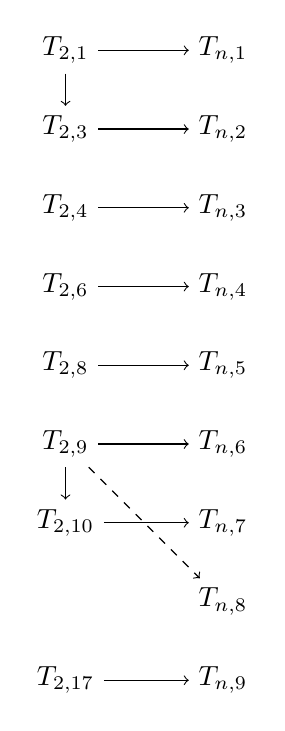
\begin{tikzpicture}
        \node (T2_1) {$T_{2,1}$};
        \node[below of=T2_1] (T2_3) {$T_{2,3}$};
        \node[below of=T2_3] (T2_4) {$T_{2,4}$};
        \node[below of=T2_4] (T2_6) {$T_{2,6}$};
        \node[below of=T2_6] (T2_8) {$T_{2,8}$};
        \node[below of=T2_8] (T2_9) {$T_{2,9}$};
        \node[below of=T2_9] (T2_10) {$T_{2,10}$};
        \node[below of=T2_10,yshift=-1cm] (T2_17) {$T_{2,17}$};

        \node[right of=T2_1, xshift=1cm] (Tn_1) {$T_{n,1}$};
        \node[below of=Tn_1] (Tn_2) {$T_{n,2}$};
        \node[below of=Tn_2] (Tn_3) {$T_{n,3}$};
        \node[below of=Tn_3] (Tn_4) {$T_{n,4}$};
        \node[below of=Tn_4] (Tn_5) {$T_{n,5}$};
        \node[below of=Tn_5] (Tn_6) {$T_{n,6}$};
        \node[below of=Tn_6] (Tn_7) {$T_{n,7}$};
        \node[below of=Tn_7] (Tn_8) {$T_{n,8}$};
        \node[below of=Tn_8] (Tn_9) {$T_{n,9}$};

        \draw[->] (T2_1) -- (Tn_1);
        \draw[->] (T2_1) -- (T2_3);
        \draw[->] (T2_3) -- (Tn_2);
        \draw[->] (T2_4) -- (Tn_3);
        \draw[->] (T2_6) -- (Tn_4);
        \draw[->] (T2_8) -- (Tn_5);
        \draw[->] (T2_9) -- (T2_10);
        \draw[->] (T2_9) -- (Tn_6);
        \draw[->, dashed] (T2_9) -- (Tn_8);
        \draw[->] (T2_10) -- (Tn_7);
        \draw[->] (T2_17) -- (Tn_9);
    \end{tikzpicture}
    \caption{Map of standard definitions to their extensions}
    \label{fig:extension-map}
\end{figure}

While the \TMS has a well-established binary form, its extension to larger alphabets introduces interpretive choices. In this work, we adopt a consistent methodology that extends all definitions equivalently. This approach ensures coherence across all extended definitions and preserves the underlying structure of the sequence. However, we acknowledge alternative constructions (such as the morphism $0\to012, 1\to02, 2\to1$ \cite{pannipitiya_2024, OEIS-A036577, OEIS-A007413, OEIS-A036585, OEIS-A036580, OEIS-A005679, OEIS-A036581, OEIS-A036582, OEIS-A036584, OEIS-A036579, OEIS-A036583, OEIS-A036586, OEIS-A036578, OEIS-A029883}) which deviate from these extensions. While these may yield sequences of interest, they do not align with the equivalence criteria established in our framework.

\subsection{Extension \arabic{extdefctr} of \TotalExtensions\xspace --- Modular Digit Sums}

This definition appears in \cite{Astudillo_2003, Dekking_2023, OEIS-TMS-3-2, Shallit_2022, Shevelev_2017, OEIS-TMS-negabinary, Starosta_2011, Parshina_2017, Robert_2013, OEIS-TMS-3, OEIS-TMS-4, OEIS-TMS-5, OEIS-TMS-6, OEIS-TMS-7, OEIS-TMS-8, OEIS-TMS-9, mcirvin_2019}.

To extend definition 1 from $2$ to $n$ players, we must first map our concept of parity to base n. We can do this by taking the parity equation defined above and replacing the $2$s with $n$, for $n \in \Integers_{\ge 2}$.

\begin{equation}
    \begin{aligned}
p_n(0) &= 0 \\
p_n(x) &= x + p_n\left(\floor{\dfrac{x}{n}}\right) \pmod{n}
    \end{aligned}
\end{equation}

Under this definition, you can construct the \TMS using the following, starting at 0:

\begin{equation}
    \edef\tempLabel{eq:pn_d\arabic{extdefctr}}
    \label{\tempLabel}
    T_{n,\arabic{extdefctr}}(x, s) = p_s(x)
\end{equation}

Note that this definition is trivially extensible to non-integer bases by redefining $p_n()$, though that is beyond the scope of this paper. This has been done in \cite{OEIS-TMS-3-2, Dekking_2023}. It has also been extended to negative integer bases \cite{OEIS-TMS-negabinary, Shallit_2022, Shevelev_2017}.

Some other works present a more generalized version, where
\begin{equation}
    t_{b,m}(n) = p_b(n) \mod{m}
\end{equation}

This allows for increased flexibility, especially when using fractional bases. In this notation, for negative integer bases, $T_{n,1}(x, s) = p_s(x) \;\; \mod{|s|}$

\subsubsection{Proof of Equivalence with Original Definition \arabic{extdefctr}}

\begin{proof}
\par\noindent\par
It is clear from visual inspection that $p_2$ is identical to our original definition of $p$.

\begin{equation}
    \begin{aligned}
                                                           p_2(x) &= p(x) \\
                         x + p_2\left(\floor{\dfrac{x}{2}}\right) &= x + p\left(\floor{\dfrac{x}{2}}\right) \\
x + \floor{\dfrac{x}{2}} + p_2\left(\floor{\dfrac{x}{2^2}}\right) &= x + \floor{\dfrac{x}{2}} + p\left(\floor{\dfrac{x}{2^2}}\right) \\
       x + \floor{\dfrac{x}{2}} + \floor{\dfrac{x}{2^2}} + \ldots &= x + \floor{\dfrac{x}{2}} + \floor{\dfrac{x}{2^2}} + \ldots
    \end{aligned}
\end{equation}
\end{proof}

This definition is also trivially extended to negative integer bases.

\stepcounter{extdefctr}
\subsection{Extended Definition \arabic{extdefctr} of \TotalExtensions\xspace --- Roots of Unity}

\begin{equation}
    \edef\tempLabel{eq:pn_d\arabic{extdefctr}}
    \label{\tempLabel}
T_{n,\arabic{extdefctr}}(x,s) = \dfrac{\log\left(\omega_s^{p_s(x)}\right)}{\log\left(\omega_s\right)}
\end{equation}

\subsubsection{Proof of Equivalence with Original Definition 3}

\begin{proof}
\par\noindent\par
    Let's start by substituting $s$ for $2$:
    \begin{equation}
    \begin{aligned}
T_{n,\arabic{extdefctr}}(x, 2) &= \dfrac{\log\left(\omega_2^{p_2(x)}\right)}{\log(\omega_2)} \\
                      &= \dfrac{\log\left((-1)^{p_2(x)}\right)}{\log(-1)} \\
                      &= \dfrac{(p_2(x) \mod{2}) \cdot \log(-1)}{\log(-1)} \\
                      &= \dfrac{(p_2(x) \mod{2}) \cdot i\pi}{i\pi} \\
                      &= p_2(x) \mod{2}
    \end{aligned}
    \end{equation}

    This is identical to $T_{2,1}$, which we earlier proved is equivalent to $T_{2,2}$.
\end{proof}

\stepcounter{extdefctr}
\subsection{Extended Definition \arabic{extdefctr} of \TotalExtensions\xspace --- Recursion}

This definition is found in \cite{schaumann_2024}, which entered preprint around the time this paper was being drafted.

\begin{equation}
\begin{aligned}
            T_{n,6}(0, s) &= 0 \\
    T_{n,6}(s \cdot x, s) &= T_{n,6}(x, s) \\
T_{n,6}(s \cdot x + k, s) &= k + T_{n,6}(x, s) \pmod{s}
\end{aligned}
\end{equation}

\subsubsection{Proof of Equivalence with Original Definition 4}

\begin{proof}
\par\noindent\par
    Let's begin by substituting $s$ for $2$:
\begin{equation}
\begin{aligned}
            T_{n,\arabic{extdefctr}}(0, 2) &= 0 \\
    T_{n,\arabic{extdefctr}}(2 \cdot x, 2) &= T_{n,\arabic{extdefctr}}(x, 2) \\
T_{n,\arabic{extdefctr}}(2 \cdot x + k, 2) &= k + T_{n,\arabic{extdefctr}}(x, 2) \pmod{2}
\end{aligned}
\end{equation}

Note that that only values for $k$ that fit in this definition are $0$ and $1$. This means we can further simplify to:
\begin{equation}
T_{n,\arabic{extdefctr}}(2 \cdot x + 1, 2) = 1 + T_{n,\arabic{extdefctr}}(x, 2) \pmod{2}
\end{equation}

This is very similar to the definition found in equation \ref{eq:p2_d4}, except that one is adding and the other subtracting. Fortunately, we know that the only values that $T_{2,4}$ will return are $0$ and $1$, which means that these operations will be completely equivalent.

\begin{align*}
1 - 0 \mod{2} &= 1 + 0 \mod{2} \\
1 - 1 \mod{2} &= 1 + 1 \mod{2}
\end{align*}
\end{proof}

\stepcounter{extdefctr}
\subsection{Extended Definition \arabic{extdefctr} of \TotalExtensions\xspace --- Highest Digit Difference}

\begin{equation}
    \edef\tempLabel{eq:pn_d\arabic{extdefctr}}
    \label{\tempLabel}
    \begin{aligned}
\text{XOR}_{n}(a, b) &= \hspace{-13pt} \sum_{i=0}^{\ceil{\log_{n}(\max(a,b) + 1)}} \hspace{-15pt} n^i \left(\floor{\dfrac{a}{n^i}} - \floor{\dfrac{b}{n^i}} \mod{n}\right) \\
       T_{n,\arabic{extdefctr}}(0, s) &= 0 \\
       T_{n,\arabic{extdefctr}}(x, s) &= \begin{aligned}[c]
           &\floor{\log_s(\text{XOR}_{s}(x, x - 1))} \\
           &+ T_{n,\arabic{extdefctr}}(x - 1, s) + 1
       \end{aligned} \pmod{s}
    \end{aligned}
\end{equation}

\note{Substitute n for 2, then simplify, plus a bit}

\subsubsection{Proof of Equivalence with Original Definition 6} ...

\stepcounter{extdefctr}
\subsection{Extended Definition \arabic{extdefctr} of \TotalExtensions\xspace --- Increment and Extend}

\note{\cite{Cai_2020} gives a good example on how to possibly adapt inversion to incrementing}

In the original version of this definition, we inverted the elements. In base $2$, this is the same thing as adding $1$ (mod $2$). Given that, let $t(x, n)$ be the first $n^x$ elements of the \ETMS, for $n \in \Integers_{\ge 2}$.

\begin{equation}
    \text{inc}(\mathbf{x}, n) = \begin{aligned}[c]
            &x_i + 1 \pmod{n} \\
            &\text{for } \mathbf{x} = (x_0, x_1, \ldots, x_{(|\mathbf{x}|-1)})
    \end{aligned}
\end{equation}

\begin{equation}
    \begin{aligned}
t(0, n) &= \tuple{0} \\
t(1, n) &= \tuple{0, 1, \ldots, n - 1} \\
t(x, n) &= t(x - 1, n) \cdot \text{inc}(t(x - 1, n), n)
    \end{aligned}
\end{equation}

Given the above, we can define a recurrence relation that will give us individual elements. It will be less efficient to compute, but will allow proofs of equivalence to be easier.

\begin{equation}
    \edef\tempLabel{eq:pn_d\arabic{extdefctr}}
    \label{\tempLabel}
    \begin{aligned}
T_{n,\arabic{extdefctr}}(0, s) &= 0 \\
T_{n,\arabic{extdefctr}}(x, s) &= T_{n,\arabic{extdefctr}}\left(x - s^{\floor{\log_s(x)}}, s\right) + 1 \pmod{s}
    \end{aligned}
\end{equation}

\subsubsection{Proof of Equivalence with Original Definition 8} ...

\stepcounter{extdefctr}
\subsection{Extended Definition \arabic{extdefctr} of \TotalExtensions\xspace --- Substitute and Flatten}

This definition appears in \cite{Chen_2019, brlek_1989, OEIS-TMS-3, OEIS-TMS-4}

\note{There's a bit of a leap here, since we have to explain why the rotation is equivalent to the binary choice presented in the original. There also might be a better syntax to define the rotation, perhaps using the format used in inv and inc.}

\begin{equation}
    \edef\tempLabel{eq:pn_d\arabic{extdefctr}}
    \label{\tempLabel}
    \begin{aligned}
            b(s) &= \tuple{0, 1, \cdots, s - 2, s - 1} \\
r(\mathbf{x}, i) &= \begin{aligned}[c]
                   &\tuple{x_{0 + i \mod{|\mathbf{x}|}}, x_{1 + i \mod{|\mathbf{x}|}}, \ldots} \\
                   &\text{for } \mathbf{x} = \tuple{x_0, x_1, \ldots, x_{(|\mathbf{x}|-1)}}
        \end{aligned} \\
         s(x, s) &= r(b(s), x) \\
            t(0) &= \tuple{0} \\
         t(x, s) &= \bigparallel_{i=0}^{2^{x-1}-1} s(t(x-1)_i, s)  \\
   T_{n,\arabic{extdefctr}}(x, s) &= t(\ceil{\log_s(x + 1)}, s)_x
    \end{aligned}
\end{equation}

\subsubsection{Proof of Equivalence with Original Definition 9} ...

\stepcounter{extdefctr}
\subsection{Extended Definition \arabic{extdefctr} of \TotalExtensions\xspace --- Recursive Rotation}

\begin{equation}
    \edef\tempLabel{eq:pn_d\arabic{extdefctr}}
    \label{\tempLabel}
    \begin{aligned}
r(\mathbf{x}, i) &= \begin{aligned}[c]
                   &\tuple{x_{0 + i \mod{|\mathbf{x}|}}, x_{1 + i \mod{|\mathbf{x}|}}, \ldots} \\
                   &\text{for } \mathbf{x} = \tuple{x_0, x_1, \ldots, x_{(|\mathbf{x}|-1)}}
        \end{aligned} \\
         t(0, s) &= \tuple{0} \\
         t(1, s) &= \tuple{0, 1, \ldots, s - 1} \\
         t(x, s) &= \bigparallel_{i=0}^{s-1} r\left(t(x-1, s), i \cdot s^{x-2}\right) \\
   T_{n,\arabic{extdefctr}}(x, s) &= t(\ceil{\log_s(x + 1)}, s)_x
    \end{aligned}
\end{equation}

\subsubsection{Proof of Equivalence with Original Definition 10} ...

\stepcounter{extdefctr}
\subsection{Extended Definition \arabic{extdefctr} of \TotalExtensions\xspace --- Latin Square Constructions}

This definition appears in \cite{tompkins_2007, Bolker_2016}

Let $L(n)$ be the reduced-form Latin Square with a first row of $\tuple{0, 1, \dots, n\!-\!1}$, and where each row progresses from one entry to the next as $L(n)_{a,x+1} \equiv L(n)_{a,x} + 1 \pmod{n}$. For each iteration $t_n$, substitute each entry $x$ for the string $L(n)_{x,*}$.

\note{Needs more explanation, largely copying from std def 8}

\begin{equation}
L(N) = \begin{pmatrix}
0 & 1 & 2 & \dots & N\!\!-\!\!1 \\
1 & 2 & \ddots & N\!\!-\!\!1 & 0 \\
2 & \ddots & N\!\!-\!\!1 & 0 & 1 \\
\vdots & N\!\!-\!\!1 & 0 & 1 & \ddots \\
N\!\!-\!\!1& 0 & 1 & \ddots & \ddots
\end{pmatrix}
\end{equation}

\subsubsection{Proof of Equivalence with Original Definition 9}

\stepcounter{extdefctr}
\subsection{Extended Definition \arabic{extdefctr} of \TotalExtensions\xspace --- Generating Functions}
\begin{equation}
\begin{aligned}
    G_s(x) &= \mathcal{G.F.} \;\; \begin{aligned}    
    \prod_{k\ge0}^\infty \sum_{i=0}^{s-1} \omega_s^i \cdot x^{i \cdot s^k}
    \end{aligned} \\
    \omega_s ^{T_{n,\arabic{extdefctr}}(j, s)} &= [x^j]G_s(x) \\
    T_{n,\arabic{extdefctr}}(j, s) &= \dfrac{\log\left([x^j]G_s(x)\right)}{\log(\omega_s)} \\
              &= \dfrac{\log\left([x^j]G_x(x)\right) \cdot s}{2i\pi} \\
\end{aligned}
\end{equation}

A similar definition to the below is found in \cite{badziahin_2015} for $x \in \mathbf{Q}((x^{-1}))$. While that definition is equivalent to $T_2$, it does not match the values for the other generalizations in this paper. For a specific example: \begin{equation}
\begin{aligned}
    T_3 &= \tuple{0,1,2,1,2,0,2,0,1,\ldots} \\
   T'_3 &= \tuple{0,2,0,2,1,0,0,0,0,\ldots} \pmod{3}
\end{aligned}
\end{equation}

\note{Above needs checking. I am only 80\% confident in my analysis here.}

\subsubsection{Proof of Equivalence with Original Definition 17}

\begin{proof}
\par\noindent\par
\textbf{Observation 1}: to start, let us rephrase definition 17 slightly

\begin{equation}
\begin{aligned}
T_{2,17}(n) &= [x^n]G(x) \\
    &= [x^n] \left(\begin{aligned}[c]
    \dfrac{\displaystyle\sum_{k\ge0}^\infty x^k - \prod_{k \ge 0}^\infty (1 - x^{2^k})}{2}
    \end{aligned}\right) \\
    &= \dfrac{[x^n] \left(\begin{aligned}[c]
    \displaystyle\sum_{k\ge0}^\infty x^k - \prod_{k \ge 0}^\infty (1 - x^{2^k})\end{aligned}\right)}{2}
     \\
    &= \dfrac{1 - [x^n]\begin{aligned}[c]
    \displaystyle\prod_{k \ge 0}^\infty (1 - x^{2^k})
    \end{aligned}
    }{2}
\end{aligned}
\end{equation}

\textbf{Observation 2}: the aparatus around the infinite product exists entirely to translate $\{1, -1\} \to \{0, 1\}$. Another way to do that is to take the complex log of this output: for $x = \{1, -1\}: \tfrac{\log(x)}{\log(-1)} = \{0, 1\}$

\textbf{Inference 1}: \begin{equation}
    \dfrac{1 - [x^n]\begin{aligned}
    \displaystyle\prod_{k \ge 0}^\infty (1 - x^{2^k})
    \end{aligned}
    }{2} = \dfrac{\log\left([x^n]\begin{aligned}
    \displaystyle\prod_{k \ge 0}^\infty (1 - x^{2^k})
    \end{aligned}\right)}{\log(-1)}
\end{equation}

\textbf{Observation 3}: $\omega_2 = -1$

\textbf{Observation 4}: If we take $T_{n,\arabic{extdefctr}}(x, s)$ for $s=2$, we get \begin{equation}
\begin{aligned}
    G_2(x) &= \mathcal{G.F.} \;\; \begin{aligned}    
    \prod_{k\ge0}^\infty \sum_{i=0}^{2-1} \omega_2^i \cdot x^{i \cdot 2^k}
    \end{aligned} \\
           &= \mathcal{G.F.} \;\; \begin{aligned}    
    \prod_{k\ge0}^\infty \omega_2^0 \cdot x^{0 \cdot 2^k} + \omega_2^i \cdot x^{i \cdot 2^k}
    \end{aligned} \\
           &= \mathcal{G.F.} \;\; \begin{aligned}    
    \prod_{k\ge0}^\infty 1 + (-1) \cdot x^{2^k}
    \end{aligned} \\
           &= \mathcal{G.F.} \;\; \begin{aligned}    
    \prod_{k\ge0}^\infty 1 - x^{2^k}
    \end{aligned}
\end{aligned}
\end{equation}
This is identical to the product found in $T_{2,17}$.

\textbf{Conclusion}: $T_{n,\arabic{extdefctr}}(x, s) = T_{2,17}(x)$
\end{proof}

\subsection{Summary}

Of the \TotalExtensions we discussed above:
\begin{itemize}
    % discovery source
    \item 1 was found on the OEIS ($T_{n,1}$)
    \item 1 was derived concurrently with another paper ($T_{n,3}$)
    \item 2 were found in another paper ($T_{n,6}, T_{n,8}$)
    \item 5 are original to this paper ($T_{n,2}, T_{n,4\dots5}, T_{n,7}, T_{n,9}$)
    \\% generating method
    \item 8 utilize recursion ($T_{n,1\dots8}$)
    \item 4 utilize floor-division ($T_{n,1\dots4}$)
    \item 4 use operations on strings, not integers ($T_{2,5\dots8}$)
    \item 0 have closed form solutions
\end{itemize}

\section{Proving Equivalence Between Extended Definitions}

\subsection{Correlating Definition 1 and Definition 2}

\begin{proof}
\par\noindent\par
    \textbf{Observation 1}: For all integers $n$, $\omega_s^n = \omega_s^{n \; \mod{s}}$

    \textbf{Inference 1}: $\dfrac{\log(\omega_s^n)}{\log(\omega_s)} = n \; \mod{s}$

    \textbf{Conclusion}: \begin{equation}
        \begin{aligned}
            T_{n,2}(x, s) &= \dfrac{\log(\omega_s^{p_s(x)})}{\log(\omega_s)} \\
                          &= \dfrac{(p_s(x) \; \mod{s}) \cdot \log(\omega_s)}{\log(\omega_s)} \\
                          &= \dfrac{(p_s(x) \; \mod{s}) \cdot 2i\pi s^{-1}}{2i\pi s^{-1}} \\
                          &= p_s(x) \; \mod{s} \\
                          &= T_{n,1}(x, s)
        \end{aligned}
    \end{equation}
\end{proof}

\subsection{Correlating Definition 4 and Definition 8}

\begin{proof}
\par\noindent\par
    \textbf{Observation 1}: For any given row of $L(N)$, it will start with the index of the row

    \textbf{Observation 2}: For any given row of $L(N)$, it will end with 1 less than the index of the row $\pmod{N}$

    \textbf{Inference 1}: $L(N)_{x,*} = r(b(N), x)$

    \textbf{Observation 3}: $T_{n,4}$ is defined as substituting $r(b(N),x)$ for each element $x$ in the previous iteration

    \textbf{Conclusion}: $T_{n,4} = T_{n,8}$
\end{proof}

\subsection{Summary}

\section{Proving Persistence (Or Lack Thereof) of Original Properties}

\subsection{Use as a Fair-Share Sequence}

\note{Goal: show that for a variety of value functions, greedy algorithms given this turn order will always minimize inequality. They should at least do so more than the standard turn order. This is going to look like setting up an equation to show}

\begin{equation}
\begin{aligned}
             eq(x, y) &= \begin{cases}
                     1& \text{if } x = y \\
                     0& \text{if } x \ne y
              \end{cases} \\
           f(v, p, s) &= \lim_{n \to \infty} \sum_{i=0}^n v(i) \cdot eq(T_n(i, s), p) \\
        \forall p : p &\in \{1, \dots, s-1\}\\
f(v, 0, s) + \epsilon &< f(v, p, s) < f(v, 0, s) - \epsilon
\end{aligned}
\end{equation}

\note{This is for $v(i)$ being a value function and $\epsilon$ being an arbitrarily small number. $f()$ is therefore the sum of total value that they will be receiving. For example, one could model a board game as $v(i) = \tfrac{1}{2^i}$, where $v()$ models the amount each turn contributes to your probability of victory. Note that this may be very hard to show for versions of $v()$ which shrink too quickly, such as $v(i) = \tfrac{1}{i!}$, so for those cases we must show that it's better than the standard turn order}

\note{$v(0)$ should always return the highest value, and $v(n)$ the lowest value, where $n+1$ is the number of items}

\subsubsection{On the value function of 1}

It is well known \cite{Cai_2020} for the Standard \TMS that
\begin{equation}
    \lim_{n\to\infty} \sum_{i=0}^n \dfrac{T_{2}(i)}{n+1} = \dfrac{1}{2}
\end{equation}

\note{Does this generalize to: ?}

\begin{equation}
    \lim_{n\to\infty} \sum_{i=0}^n\dfrac{T_{n}(i, s)}{n+1} = \sum_{i=0}^{s-1}\dfrac{i}{s} = \dfrac{n-1}{2}
\end{equation}

\note{and}

\begin{equation}
\begin{aligned}
    &\forall{x} \;|\; 0 \le x < s \text{ and } x \in \mathbf{Z} \\
    &\lim_{n\to\infty} \sum_{i=0}^n\dfrac{eq\left(T_{n}(i, s), x\right)}{n+1} = \dfrac{1}{s}
\end{aligned}
\end{equation}

\subsubsection{Galois Duels \& Related Decreasing Functions}

The OEIS Sequence A287150 \cite{cooper_2011, OEIS-A287150} gives an extension of $T_{2,21}$ for 3 players. It should be noted that it is different from the extensions in this paper, meaning that this property is not preserved. \begin{equation}
\begin{aligned}
    T_3 &= \tuple{0, 1, 2, 1, 2, 0, 2, 0, 1, \dots} \\
A287150 &= \tuple{0, 1, 2, 2, 1, 0, 2, 1, 0, \dots}
\end{aligned}
\end{equation}

\subsubsection{Uniform Distributions}

Let us have a value function that goes over a uniform distribution:

\begin{equation}
    v_u(x) = a+(b-a)(1-\dfrac{x}{n})
\end{equation}
Where \begin{itemize}
    \item $a$ is the lower bound of the distribution
    \item $b$ is the upper bound of the distribution, and
    \item $n$ is the total number of items
\end{itemize}

\begin{conjecture}
\label{conj:equit_dist_uniform}
For $n \ge 2$ players and $n^k$ items, greedily distributing items in the order $T_n$ will minimize the difference between players' received values, when values are distributed according to $v_u(x)$.
\end{conjecture}

\subsubsection{Normal Distributions}

Let us have a value function that goes over a normal distribution:

\begin{equation}
    v_n(x) =\mu-\sigma \cdot \Phi^{-1}\left(\dfrac{x}{n}\right)
\end{equation}
Where \begin{itemize}
    \item $\mu$ is the mean of the distribution
    \item $\sigma$ is the standard deviation, and
    \item $\Phi^{-1}$ is inverse CDF of the normal distribution
\end{itemize}

\begin{conjecture}
\label{conj:equit_dist_normal}    
For $n \ge 2$ players and $n^k$ items, greedily distributing items in the order $T_n$ will minimize the difference between players' received values, when values are distributed according to $v_n(x)$.
\end{conjecture}

\subsubsection{Exponential Distributions}

Let us have a value function that goes over an exponential distribution:

\begin{equation}
    v_e(x) = -\dfrac{1}{\lambda} \cdot \ln\left(1 - \dfrac{x}{n}\right)
\end{equation}
Where $\lambda$ is the rate parameter of the exponential distribution

\begin{conjecture}
\label{conj:equit_dist_exponential}
For $n \ge 2$ players and $n^k$ items, greedily distributing items in the order $T_n$ will minimize the difference between players' received values, when values are distributed according to $v_e(x)$.
\end{conjecture}

\subsubsection{Discrete Value Distributions}

It is trivial to show that for non-continuous value functions, neither the Standard nor Extended \TMS distributed fairly. For example, consider a set of items with the value $\{2^5, 2^3, 2^3, 1, 1, 1\}$. When split among two players, they will end up with a total value of $\tuple{34, 17}$. A more equitable distribution is achieved by giving player $0$ the first item, and the remainder to player $1$, resulting in $\tuple{32, 19}$. Similar observations can be made for larger numbers of players. This is left to the reader.

\subsection{Palindrome}

In base 2: \begin{equation}
    \forall x, y : (x > 1) \land (0 \le y < 2^x), \;\; t_2(x)_y = t_2(x)_{2^x - y - 1}
\end{equation}
\note{(Find a citation for this)}

\begin{proof}
\par\noindent\par
    \textbf{Assumption 1}: $n > 2$

    \textbf{Assumption 2}: $t_n(x)$ is palindromic, for $x > 1$

    \textbf{Observation 1}: $$t_n(x)_{n^x - 1} = p_n(n^x - 1) \equiv (n - 1)x \pmod{n}$$

    \textbf{Inference 1}: By Assumption 2, $t_n(x)_0 = 0 = t_n(x)_{n^x - 1}$

    \textbf{Observation 2}: $$t_n(x)_{n^x - 2} = p_n(n^x - 2) \equiv (n - 1)(x - 1) - 2 \pmod{n}$$

    \textbf{Inference 2}: By Assumption 2, $t_n(x)_1 = 1 = t_n(x)_{n^x - 2}$

    \textbf{Inference 3}: By Inferences 1 \& 2, \begin{equation}\begin{aligned}
        t_n(x)_{n^x-1} &\equiv t_n(x)_{n^x-2} - 1  \\
        (n - 1)x &\equiv (n - 1)(x - 1) - 2 - 1 \\
                 &\equiv (n - 1)(x - 1) + (n - 1) - 2 \\
                 &\equiv (n - 1)x - 2 \\
               0 &\equiv - 2 \\
    \end{aligned}
    \end{equation}

    \textbf{Contradiction!} While $n > 2$, these terms cannot be equal. This means that if the first and last terms match, the second and penultimate will not, and vice versa.
\end{proof}

\subsection{Uniform Recurrence}

\note{The \TMS is a uniformly recurrent word: given any finite string X in the sequence, there is some length nX (often much longer than the length of X) such that X appears in every block of length nX. Tackle this by using $T_{n,6}$}

\subsection{Deriving Square Free Sequences}

\note{Given a word $X : |X| > 1, X \in T_n$, $(X \concat X) \not\in T_n$. Square Free implies Overlap Free. The original \TMS is \textit{not} square-free, as it is not possible to construct a square-free sequence with an alphabet smaller than 3 (cite to Thue himself). However it can produce a square-free sequence easily by taking the difference of subsequent terms (A029883).}

Let $T_{dn}$ be the sequence generated by taking the difference of terms in the sequence $T_n$, such that $T_{d2} = \tuple{-1, 0, 1, -1, \ldots}$. The resulting sequence is square-free.

\begin{theorem}
\label{theo:square_free_dn}
This method does not generalize to $n \in \Integers_{\ge2}$
\begin{proof}
\par\noindent\par Proof by counterexample: \begin{itemize}
    \item $T_{d3}(19\dots25) = \tuple{-1, 1, -1, -1, 1, -1}$
    \item $T_{d4}(37\dots45) = \tuple{-1, -1, 2, -1, -1, -1, 2, -1}$
    \item $\forall n : n > 4,\; T_{dn}(0\dots3) = \tuple{-1,-1,-1,-1}$
\end{itemize}
\end{proof}
\end{theorem}

Another method to make a square-free sequence from $T_2$ is to construct a different alphabet \cite{offner_repetitions} using pairs of terms. This generates a new sequence $T_{p2} = \tuple{01, 11, 10, 01, 10, 00, \dots}$

\begin{conjecture}
\label{conj:square_free_pn} 
This method generalizes to $T_n$ by iterating pairwise, making $T_{pn}$, where $T_{pn}(x) = \tuple{T_n(x), T_n(x+1)}$.
\end{conjecture}

\begin{proof}
    \note{Not sure how to do this rigorously, but computer testing hasn't found a counterexample}
\end{proof}

\begin{conjecture}
\label{conj:square_free_nxn}
This method generalizes to $T_n$ by iterating over a sliding window of size $n$, making $T_{n\times n}$, where $T_{n\times n}(x) = \tuple{T_n(x), T_n(x+1), \dots, T_n(x+n-1)}$.
\end{conjecture}

\begin{proof}
    \note{Not sure how to do this rigorously, but computer testing hasn't found a counterexample}
\end{proof}

\subsection{Overlap Free}

Extensions of the \TMS that comply with $T_{n,8}$ are overlap-free \cite{tompkins_2007}. \note{Is that true? I thought they used invertible matrices in this paper, and I don't think the general solution in $T_{n,8}$ are invertible. Needs followup.}

\note{Given a word $X : |X| > 1, X \in T_n$, $(X \concat X \concat X_0) \not\in T_n$. For $T_2$, this is shown in \cite{pannipitiya_2024}. Note additionally that this apparently is equivalent to 7/3-power-free \cite{rampersad_2003}. Overlap Free implies Cube Free}

\subsection{Cube Free}

Because extensions of the \TMS that comply with $T_{n,8}$ are overlap-free \cite{tompkins_2007}, they are also cube-free.

\note{Given a word $X : |X| > 1, X \in T_n$, $(X \concat X \concat X) \not\in T_n$.}

\subsection{Aperiodicity}

\note{Not totally sure how this should go, but I think a good approximation would be to show that the distance between the nearest two appearances of a substring grows to infinity much faster than the length of those substrings grows. For words of size greater than $n$, this seems feasible. For words in size $2$ thru $n$, I think I need to show that the distance between repetitions is aperiodic. That \textit{should} be equivalent to distance between repetitions of integers, since one of the definitions expands digits to words}

\subsection{Generalization of Prouhet-Terry-Escott Problem}

The standard Prouhet-Terry-Escott problem \cite{Adler_1977, prouhet_1851} is

\begin{quote}
    Given $m > 1$ find $r > m$ and disjoint sets of distinct integers $\{a_1 \dots a_r\}$ and $\{b_1 \dots b_r\}$ such that:
    \begin{equation}
        \sum_{i=1}^r a_i^k = \sum_{i=1}^r b_i^k
    \end{equation}
    holds for every $k = 1 \dots m$
\end{quote}

Does this extension allow us to generalize to 

\begin{quote}
    Given $m > 1$ find $r > m$ and $n$ disjoint sets of distinct integers $\{s_{1,1} \dots s_{1,r}\}$, $\{s_{2,1} \dots s_{2,r}\}$, $\dots$, $\{s_{n,1} \dots s_{n,r}\}$ such that:
    \begin{equation}
        \forall x : 2 \le x \le n \left(\sum_{i=1}^r s_{1,i}^k = \sum_{i=1}^r s_{x,i}^k \right)
    \end{equation}
    holds for every $k = 1 \dots m$
\end{quote}

\note{I \textit{think} \cite{Bolker_2016} says yes, but I'm not certain I understand it yet}

\subsection{Maresh Multifractions}

It is a well known result \cite{Allouche-Shallit_1999} that the infinite nested fraction defined by: \begin{equation}
    \dfrac{1}{2} \to \dfrac{\left(\dfrac{1}{2}\right)}{\left(\dfrac{3}{4}\right)} \to \dfrac{\left(\dfrac{\left(\tfrac{1}{2}\right)}{\left(\tfrac{3}{4}\right)}\right)}{\left(\dfrac{\left(\tfrac{5}{6}\right)}{\left(\tfrac{7}{8}\right)}\right)} \to \dots \to \prod_{k=1}^\infty k^{(-1)^{T_2(k-1)}}
\end{equation}

and that this converges to $\tfrac{1}{\sqrt{2}}$. Can we generalize fractions in a way that this result holds for $T_n$?

Let a Maresh multifraction \cite{mcirvin_2019} be

\begin{equation}
M_n(a_0, \dots, a_{n-1}) = \prod_{k=0}^{n-1} a_{k}^{e^{2ki \pi/n}}
\end{equation}

Note that in the case of $n=2$, this reduces to a standard fraction: $M_2(a, b) = \tfrac{a}{b}$. For all other cases, it rotates the input values such that they are equidistant around the unit circle, then takes their product.

\begin{conjecture}
\label{conj:maresh_multifraction}
Suppose for some multifraction of size $n$, we begin chunking the counting numbers into groups of $n$. Each of these groups then gets put into a multifraction, and these multifractions subsequently get put into a multifraction, and so on. We will call this sequence $F_n$
\begin{equation}
\begin{aligned}
   F_n &= \lim_{x\to\infty} F_n(x) \\
F_n(1) &= M_n(1, \ldots, n-1) \\
F_n(2) &= M_n\left(\begin{aligned}
        &M_n(1, \ldots, n), \\
        &M_n(n+1, \ldots, 2n),\\ 
        &\ldots, \\
        &M_n((n-1)n+1, \ldots, n^2)
\end{aligned}\right)\\
   \forall n: n &\ge 2, |F_n| = \left| \sum_{k=0}^\infty (k+1)(\omega_n^{T_n(k)}) \right| = \dfrac{1}{\sqrt{n}}
\end{aligned}
\end{equation}
\end{conjecture}

\subsection{Fractal Turtle Geometry}

\note{$T_2$ generates the von Koch snowflake. Do other integer bases also generate fractals in a way that can be generalized? \cite{mcirvin_2019, schaumann_2024}}

\section{Acknowledgment}

We thank Dan Rowe for helping with the initial work on this paper, as well as Randy Appleton and Lydia Crocker who helped greatly with proofreading and editing.

\section{Future Work}

While this paper is intended to be as comprehensive as possible, there are still many things left to analyze. \note{Fill in with anything I didn't get to from notes}

\subsection{Open Conjectures}

The following conjectures were not able to be definitively proven or disproven in this paper. They have been computationally tested to the best our resources can handle.

\begin{itemize}
    \item \textbf{Conjecture \ref{conj:equit_dist_uniform}} --- $T_n$ distributes values equitably when values are determined by $v_u(x)$
    \item \textbf{Conjecture \ref{conj:equit_dist_normal}} --- $T_n$ distributes values equitably when values are determined by $v_n(x)$
    \item \textbf{Conjecture \ref{conj:equit_dist_exponential}} --- $T_n$ distributes values equitably when values are determined by $v_e(x)$
    \item \textbf{Conjecture \ref{conj:square_free_pn}} --- $T_{pn}$ is square free
    \item \textbf{Conjecture \ref{conj:square_free_nxn}} --- $T_{n \times n}$ is square free
    \item \textbf{Conjecture \ref{conj:maresh_multifraction}} --- The Magnitude of the Maresh Multifraction $F_n$ converges to $\tfrac{1}{\sqrt{n}}$
\end{itemize}

\subsection{Negative Bases}

There are existing extensions that deal with negative bases \cite{OEIS-TMS-negabinary}. To what extent can those be harmonized with the extensions in this paper?

\subsection{Rational Bases}

There are existing extensions that deal with rational bases \cite{OEIS-TMS-3-2}. To what extent can those be harmonized with the extensions in this paper?

\subsection{Claims about the Standard \TMS}

These claims are found in \cite{OEIS-TMS}.

\begin{conjecture}
    \begin{equation}    
    \forall x : x\ge 0, T_2(\text{A004760}(x+1)) = 1 - T_2(x)
    \end{equation}
\end{conjecture}

\begin{conjecture}
    \begin{equation}
        \forall x : x \ge 0, T_2(\text{A160217}(x)) = 1 - T_2(x)
    \end{equation}
\end{conjecture}

\begin{conjecture}
    \begin{equation}
        \mathcal{G.F.}\;\; A(x) \text{ satisfies}: A(x) = \dfrac{x}{1 - x^2} + (1 - x) \cdot A(x^2)
    \end{equation}
\end{conjecture}

\begin{conjecture}
    \begin{equation}
         T_2((2^m-1)^2) = \dfrac{1-(-1)^m}{2}
    \end{equation}
\end{conjecture}

\subsection{Claims about the Inverted \TMS $\tuple{1, 0, 0, 1, \dots}$}

These claims are found in \cite{OEIS-TMS-inv}.

\begin{conjecture}
    \begin{equation}
    \begin{aligned}
        \text{If } A(n) &= (a(0),a(2),...,a(2^n-1)), \\
        \text{ then } A(n+1) &= (A(n),1-A(n)), \\
        \text{where } T_2 &= 1 - [x^n]A(x)
    \end{aligned}
    \end{equation}
\end{conjecture}

\subsection{Claims about the Signed \TMS $\tuple{1, -1, -1, 1, \dots}$}

These claims are found in \cite{OEIS-TMS-pos-neg}.

\begin{conjecture}
    \begin{equation}
    \begin{aligned}
        \mathcal{G.F.}\; A(x) \text{ makes } 0 &= f(A(x), A(x^2), A(x^4)) \\
        \text{where } f(u, v, w) &= v^3 - 2uvw + u^2w\\
        \text{and } T_2(n) &= \dfrac{1 - [x^n]A(x)}{2}
    \end{aligned}
    \end{equation}
\end{conjecture}

\begin{conjecture}
    \begin{equation}
    \begin{aligned}
        \mathcal{G.F.}\; A(x) \text{ makes } 0 &= f(A(x), A(x^2), A(x^3), A(x^6))\\
        \text{where } f(a, b, c, d) &= a^3d - 3a^2bd + 3ab^2d - b^3c\\
        \text{and } T_2(n) &= \dfrac{1 - [x^n]A(x)}{2}
    \end{aligned}
    \end{equation}
\end{conjecture}

\begin{conjecture}
    \begin{equation}
        (-1)^{T_2(n)} = \dfrac{B_n(\!-\!\text{A038712}(1) \!\cdot\! 0!, \dots, \!-\!\text{A038712}(n) \!\cdot\! (n\!\!-\!\!1)!)}{n!}
    \end{equation}
    Where \begin{itemize}
        \item $B_n(x_1, ..., x_n)$ is the $n$-th complete Bell polynomial
        \item A038712 \cite{OEIS-A038712} is $a(n) = 2^{\text{A007814}(n)+1}-1$
        \item A007814 \cite{OEIS-A007814} is the exponent of highest power of 2 dividing $n$
    \end{itemize}
\end{conjecture}

\begin{conjecture}
    \begin{equation}
        \forall x : x \ge 0, (-1)^{T_2(x)} = \text{A008836}(\text{A005940}(1+x))
    \end{equation}
    Where: \begin{itemize}
        \item A008836 \cite{OEIS-A008836} is Liouville's function $\lambda(n) = (-1)^k$, where $k$ is number of primes dividing $n$ (counted with multiplicity)
        \item A005940 \cite{OEIS-A005940} is the Doudna sequence
    \end{itemize}
\end{conjecture}

\subsection{Claims about the Standard \ETMS For $n=3$}

These claims are found in \cite{OEIS-TMS-3}.

\begin{conjecture}
    \begin{equation}
        \forall x : x \ge 0, T_3(x) = \text{A026600}(x+1) - 1
    \end{equation}
    where \begin{itemize}
        \item A026600 \cite{OEIS-A026600} $a(n)$ is the $n$-th letter of the infinite word generated from $w(1)=1$ inductively by $w(n)=\text{JUXTAPOSITION}\{w(n-1),w'(n-1),w"(n-1)\}$, where $w(k)$ becomes $w'(k)$ by the cyclic permutation $1\to2\to3\to1$ and $w"(k) = (w')'(k)$.
    \end{itemize}
\end{conjecture}

\section{Appendix 1 --- Other Considered Extensions}

There are a number of extensions that don't meet the strict standard of mutual equivalence laid out in this paper, but are nonetheless worthy of mention.

\subsection{Honorable Mention --- Square Free Ternary Sequences}

A family of sequences commonly derived from the \TMS is the morphism $a\to abc, b\to ac, c\to b$, with various substitutions of the letters \cite{pannipitiya_2024, OEIS-A036577, OEIS-A007413, OEIS-A036585, OEIS-A036580, OEIS-A005679, OEIS-A036581, OEIS-A036582, OEIS-A036584, OEIS-A036579, OEIS-A036583, OEIS-A036586, OEIS-A036578, OEIS-A029883}. They have the wonderful property of begin among the smallest square-free sequences, as measured by alphabet size. This generates sequences like: \begin{itemize}
    \item $\tuple{2, 1, 0, 2, 0, 1, 2, 1, 0, \dots}$ \cite{pannipitiya_2024, OEIS-A036577} ($2\!\to\!210, \!1\!\to\!20, 0\!\to\!1$)
    \item $\tuple{1, 2, 3, 1, 3, 2, 1, 2, 3, \dots}$ \cite{OEIS-A007413} ($1\!\to\!123, 2\!\to\!13, 3\!\to\!2$)
    \item $\tuple{3, 2, 1, 3, 1, 2, 3, 2, 1, \dots}$ \cite{OEIS-A036585} ($3\!\to\!321, 2\!\to\!31, 1\!\to\!2$)
    \item $\tuple{0, 1, 2, 0, 2, 1, 0, 1, 2, \dots}$ \cite{OEIS-A036580} ($0\!\to\!012, 1\!\to\!02, 2\!\to\!1$)
    \item $\tuple{2, 1, 3, 2, 3, 1, 2, 1, 3, \dots}$ \cite{OEIS-A005679} ($2\!\to\!213, 1 \!\to\! 23, 3\!\to\!1$)
    \item $\tuple{0, 2, 1, 0, 1, 2, 0, 2, 1, \dots}$ \cite{OEIS-A036581} ($0\!\to\!021, 2\!\to\!01, 1\!\to\!2$)
    \item $\tuple{2, 3, 1, 2, 1, 3, 2, 3, 1, \dots}$ \cite{OEIS-A036582} ($2\!\to\!231, 3\!\to\!21, 1\!\to\!3$)
    \item $\tuple{3, 1, 2, 3, 2, 1, 3, 1, 2, \dots}$ \cite{OEIS-A036584} ($3\!\to\!312, 1\!\to\!32, 2\!\to\!1$)
    \item $\tuple{1, 2, 0, 1, 0, 2, 1, 2, 0, \dots}$ \cite{OEIS-A036579} ($1\!\to\!120, 2\!\to\!10, 0\!\to\!2$)
    \item $\tuple{1, 3, 2, 1, 2, 3, 1, 3, 2, \dots}$ \cite{OEIS-A036583} ($1\!\to\!132, 3\!\to\!12, 2\!\to\!3$)
    \item $\tuple{2, 0, 1, 2, 1, 0, 2, 0, 1, \dots}$ \cite{OEIS-A036586} ($2\!\to\!201, 0\!\to\!21, 1\!\to\!0$)
    \item $\tuple{1, 0, 2, 1, 2, 0, 1, 0, 2, \dots}$ \cite{OEIS-A036578} ($1\!\to\!102, 0\!\to\!12, 2\!\to\!0$)
    \item $\tuple{1, 0, \!-\!1, 1, \!-\!1, 0, 1, 0, \dots}$\hspace{2pt} \cite{OEIS-A029883} ($1\!\to\!10\!\!-\!\!1, 0\!\to\!1\!\!-\!\!1, \!-\!1\!\to\!0$)
\end{itemize}

\subsection{A071858, A051329}

These sequences \cite{OEIS-A071858, OEIS-A051329} are of the form 
\begin{equation}
a(n) = p_s(n) \pmod{s + 1}
\end{equation}
In the notation of some other papers, they are $t_{2,3}$ and $t_{3,4}$, respectively.

\subsection{A005681}

\subsection{A239110}

\subsection{A317189}

\subsection{A089215}

\subsection{A029884}

\section{Appendix 2 --- General Performance Results}

\begin{figure}[H]
    \centering
    \vspace{-20pt}
    \caption{Benchmark results up to seconds.}
    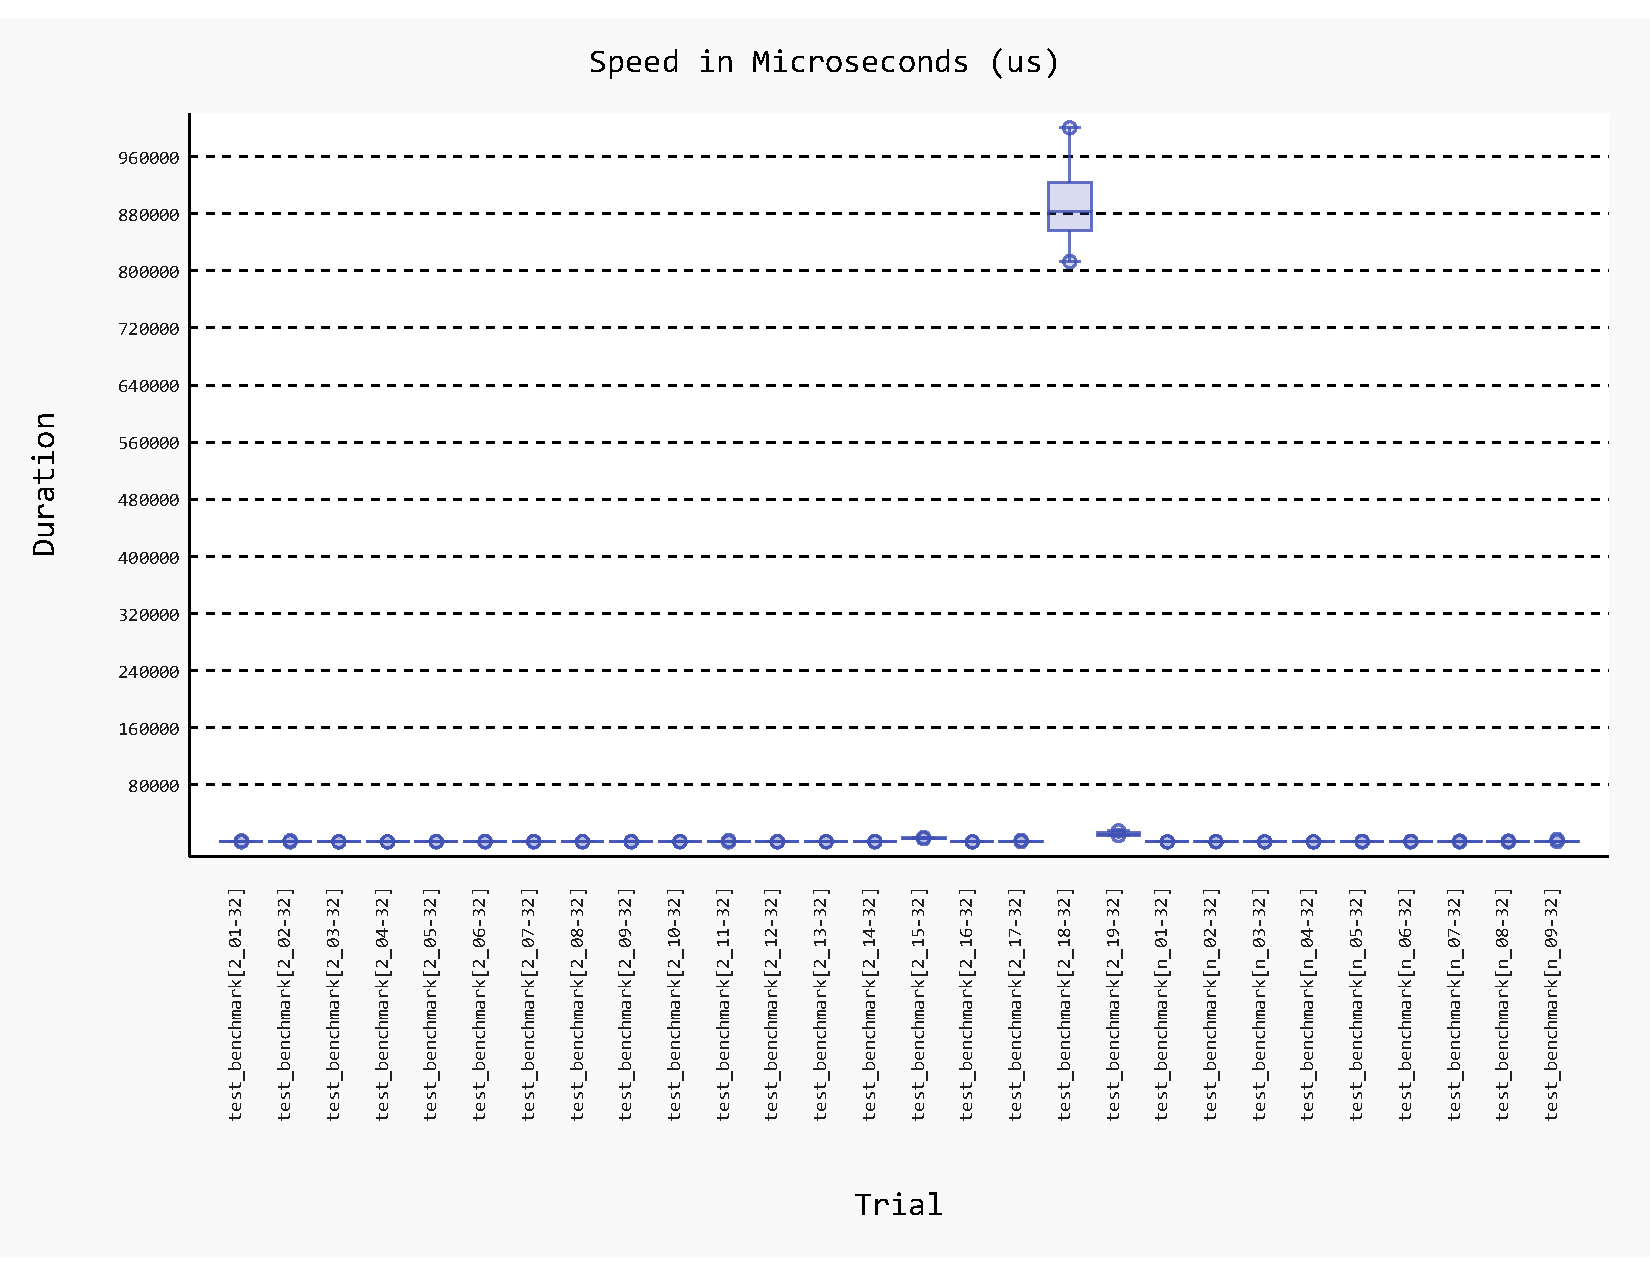
\includegraphics[width=\linewidth, trim=0 0 0 0, clip]{figures/benchmark/20241204_182753.pdf}
    \label{fig:benchmark_in_s}
    \vspace{-25pt}
\end{figure}

\begin{figure}[H]
    \centering
    \vspace{-20pt}
    \caption{Benchmark results up to milliseconds.}
    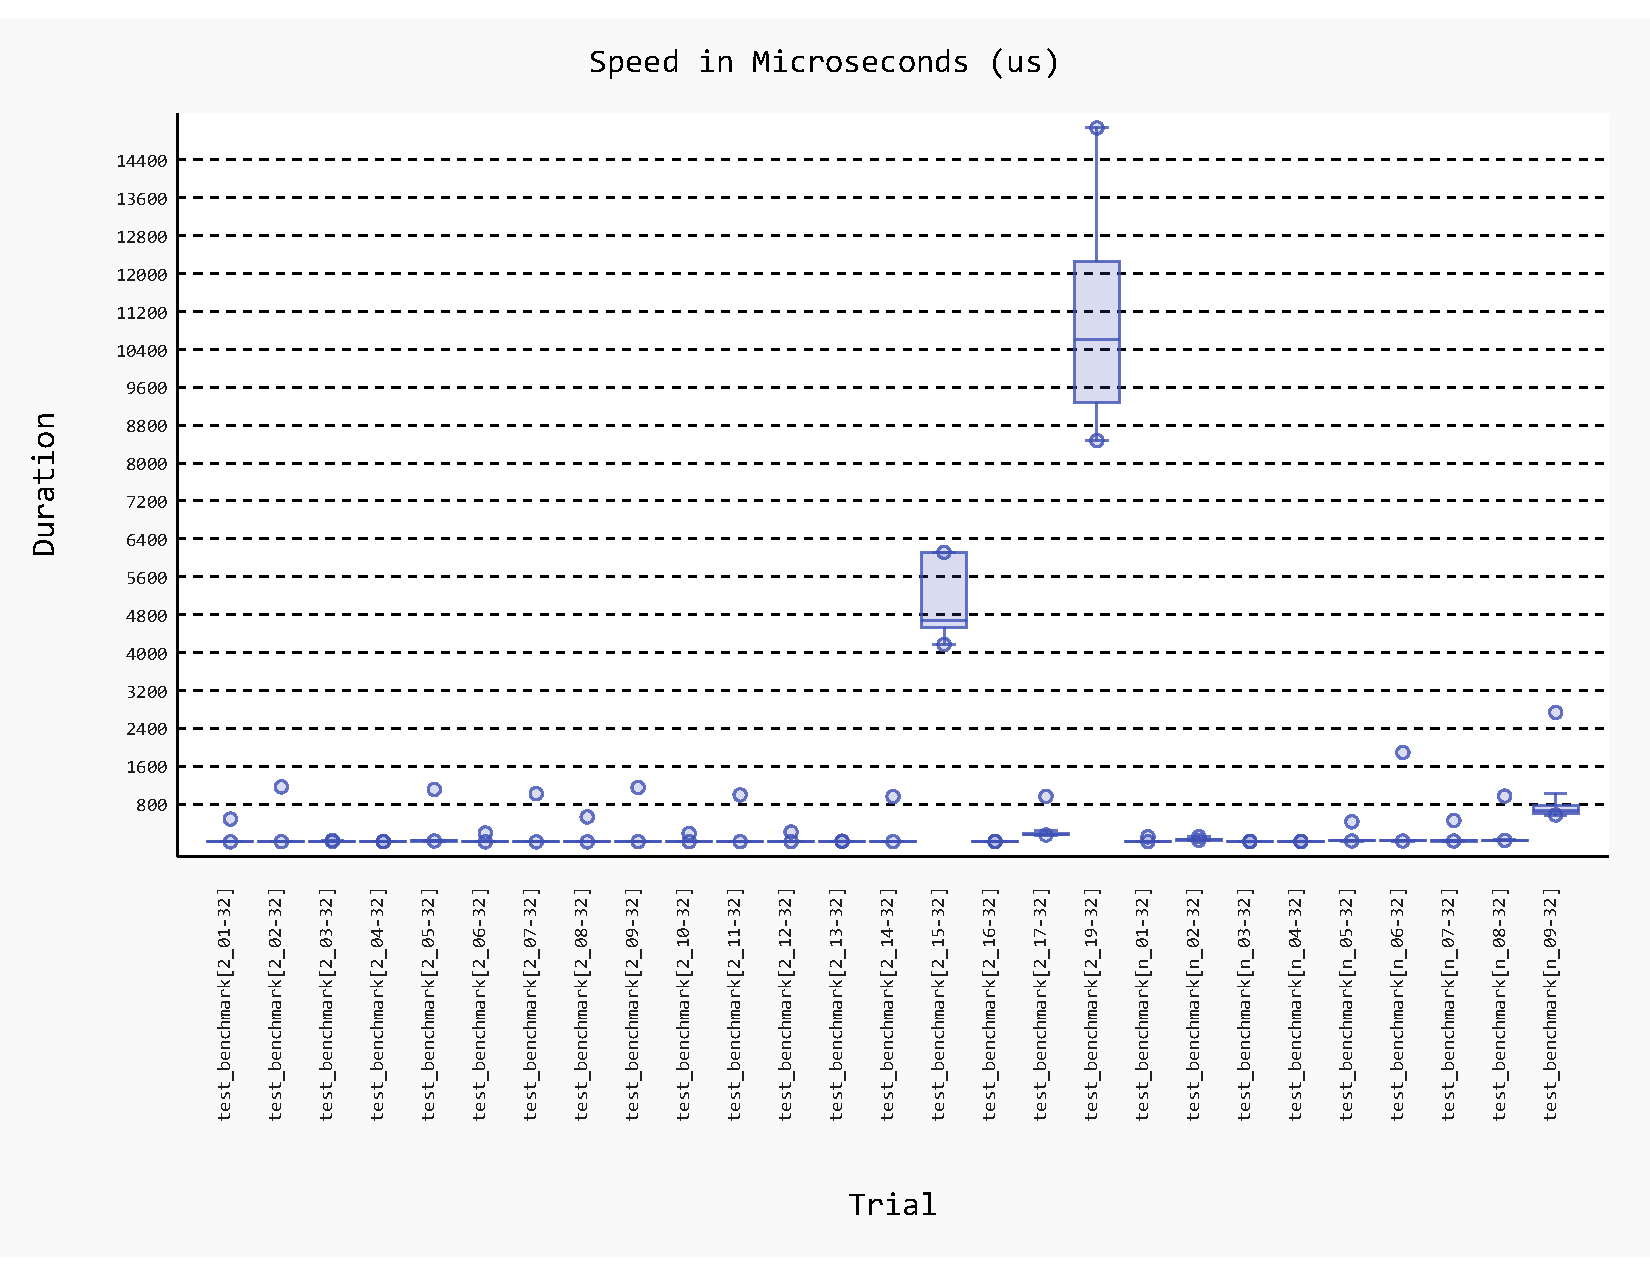
\includegraphics[width=\linewidth, trim=0 0 0 0, clip]{figures/benchmark/20241204_182830.pdf}
    \label{fig:benchmark_in_ms}
    \vspace{-25pt}
\end{figure}

\begin{figure}[H]
    \centering
    \vspace{-20pt}
    \caption{Benchmark results up to microseconds.}
    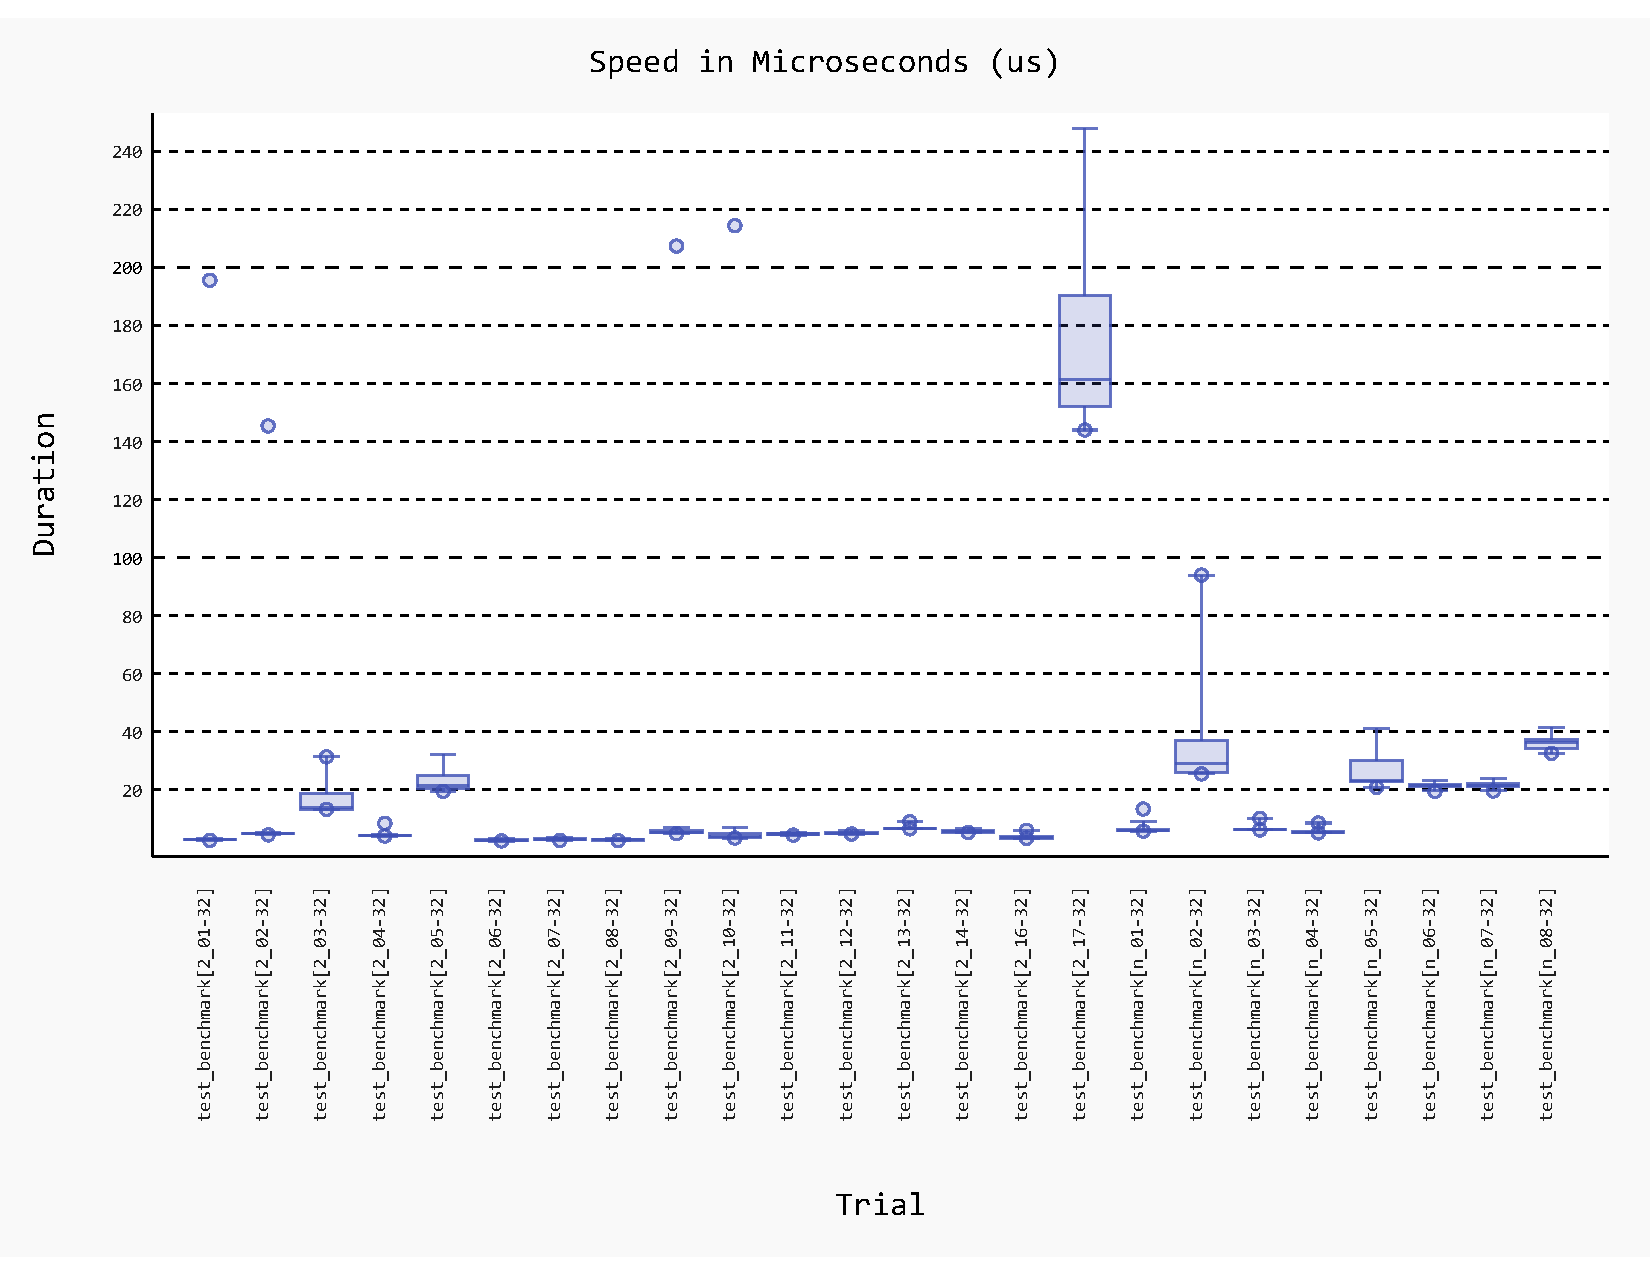
\includegraphics[width=\linewidth, trim=0 0 0 0, clip]{figures/benchmark/20241204_183033.pdf}
    \label{fig:benchmark_in_us}
    \vspace{-25pt}
\end{figure}

\begin{figure}[H]
    \centering
    \vspace{-20pt}
    \caption{Compared Complexity for Fixed Size Integers and One Element.}
    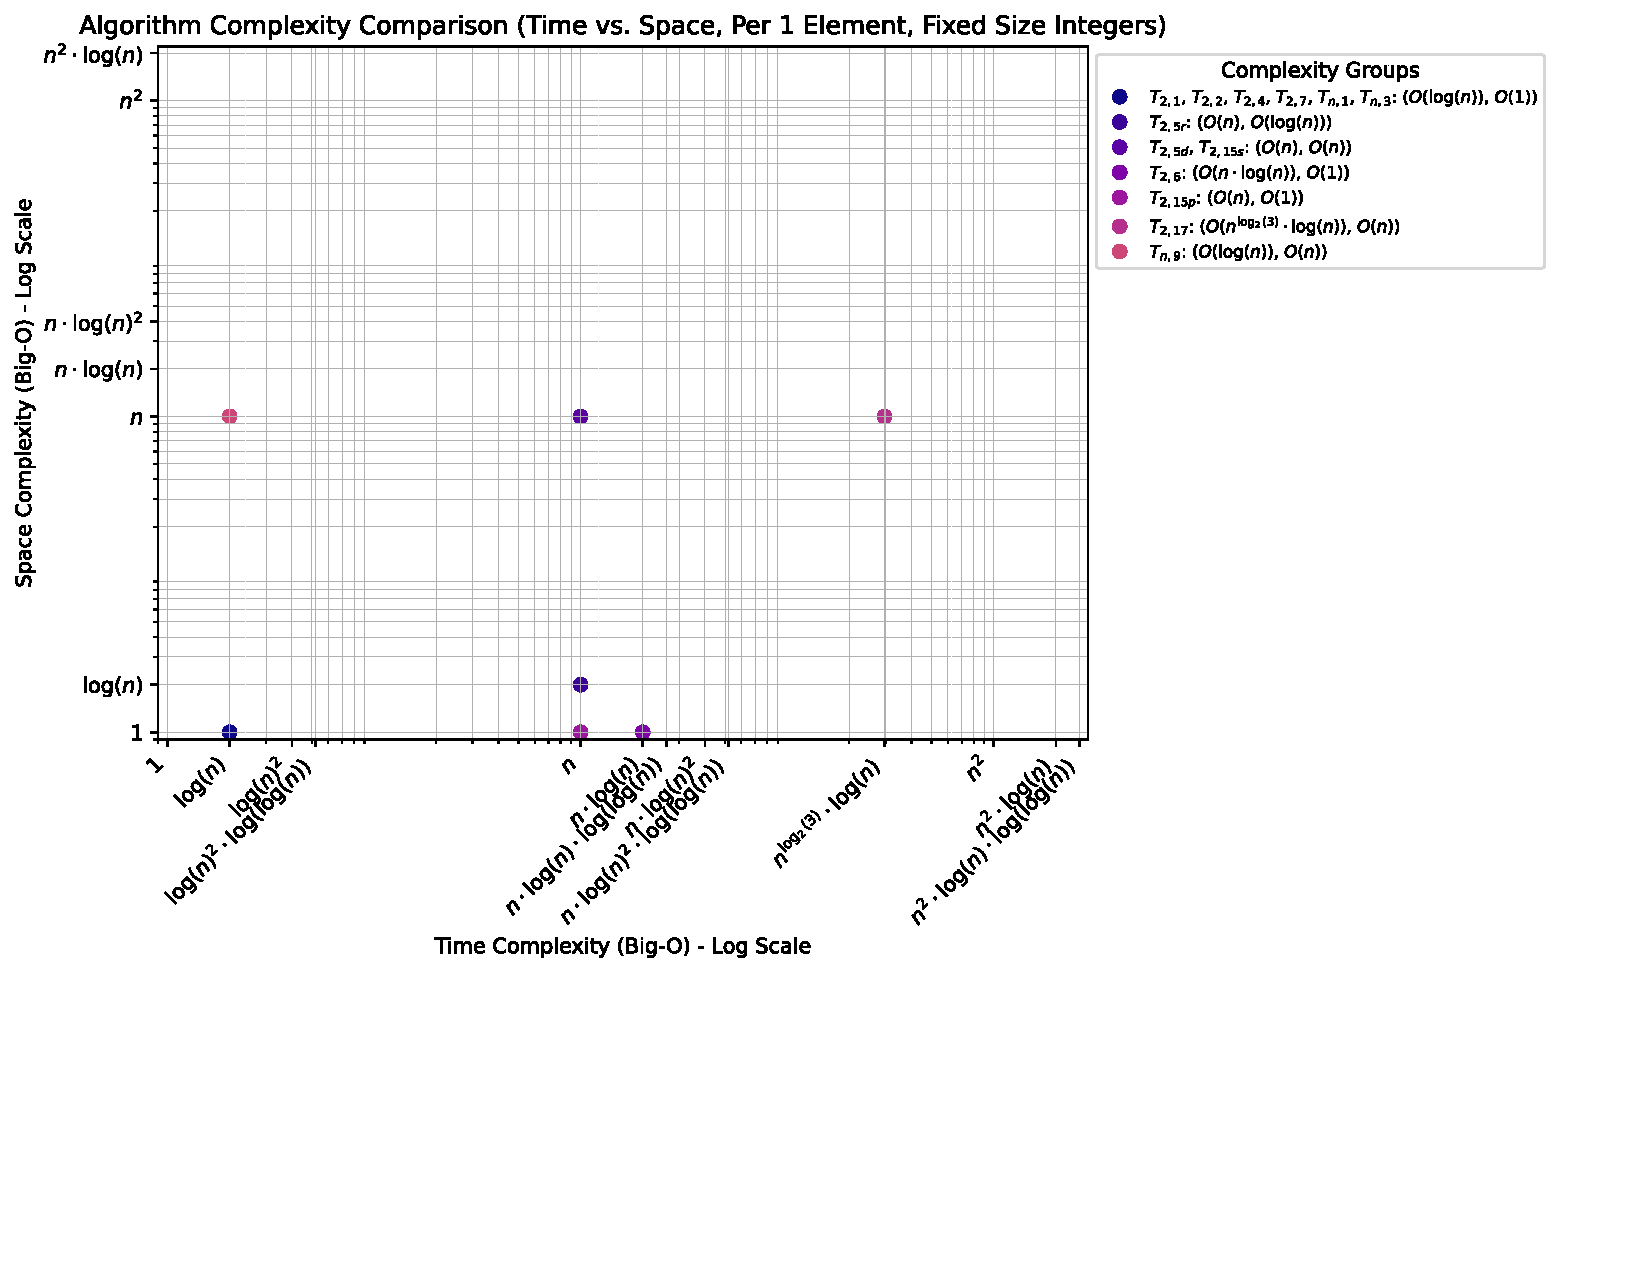
\includegraphics[width=\linewidth, trim=0 0 0 0, clip]{figures/complexity/complexity_comparison_0_0.pdf}
    \label{fig:complexity_0_0}
    \vspace{-25pt}
\end{figure}

\begin{figure}[H]
    \centering
    \vspace{-20pt}
    \caption{Compared Complexity for Fixed Size Integers and $n$ Elements.}
    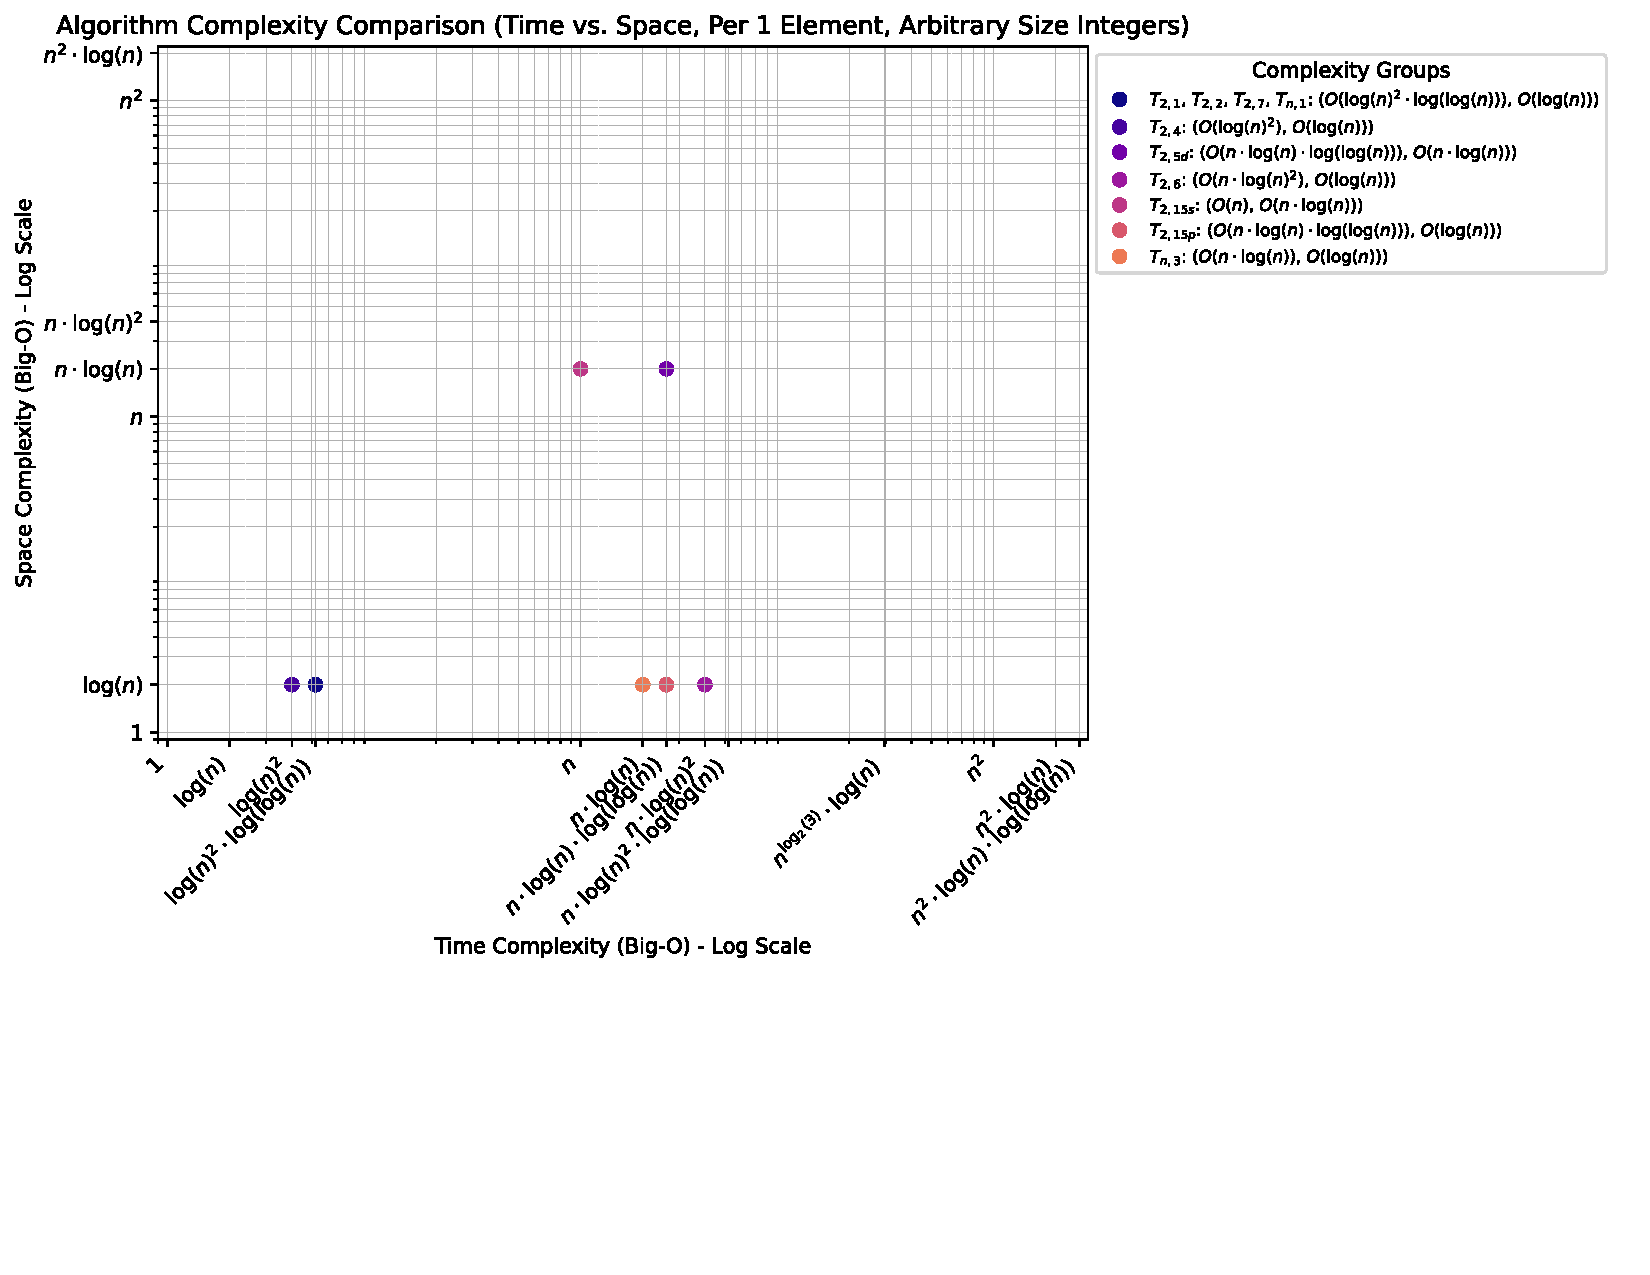
\includegraphics[width=\linewidth, trim=0 0 0 0, clip]{figures/complexity/complexity_comparison_0_1.pdf}
    \label{fig:complexity_0_1}
    \vspace{-25pt}
\end{figure}

\begin{figure}[H]
    \centering
    \vspace{-20pt}
    \caption{Compared Complexity for Arbitrary Size Integers and One Element.}
    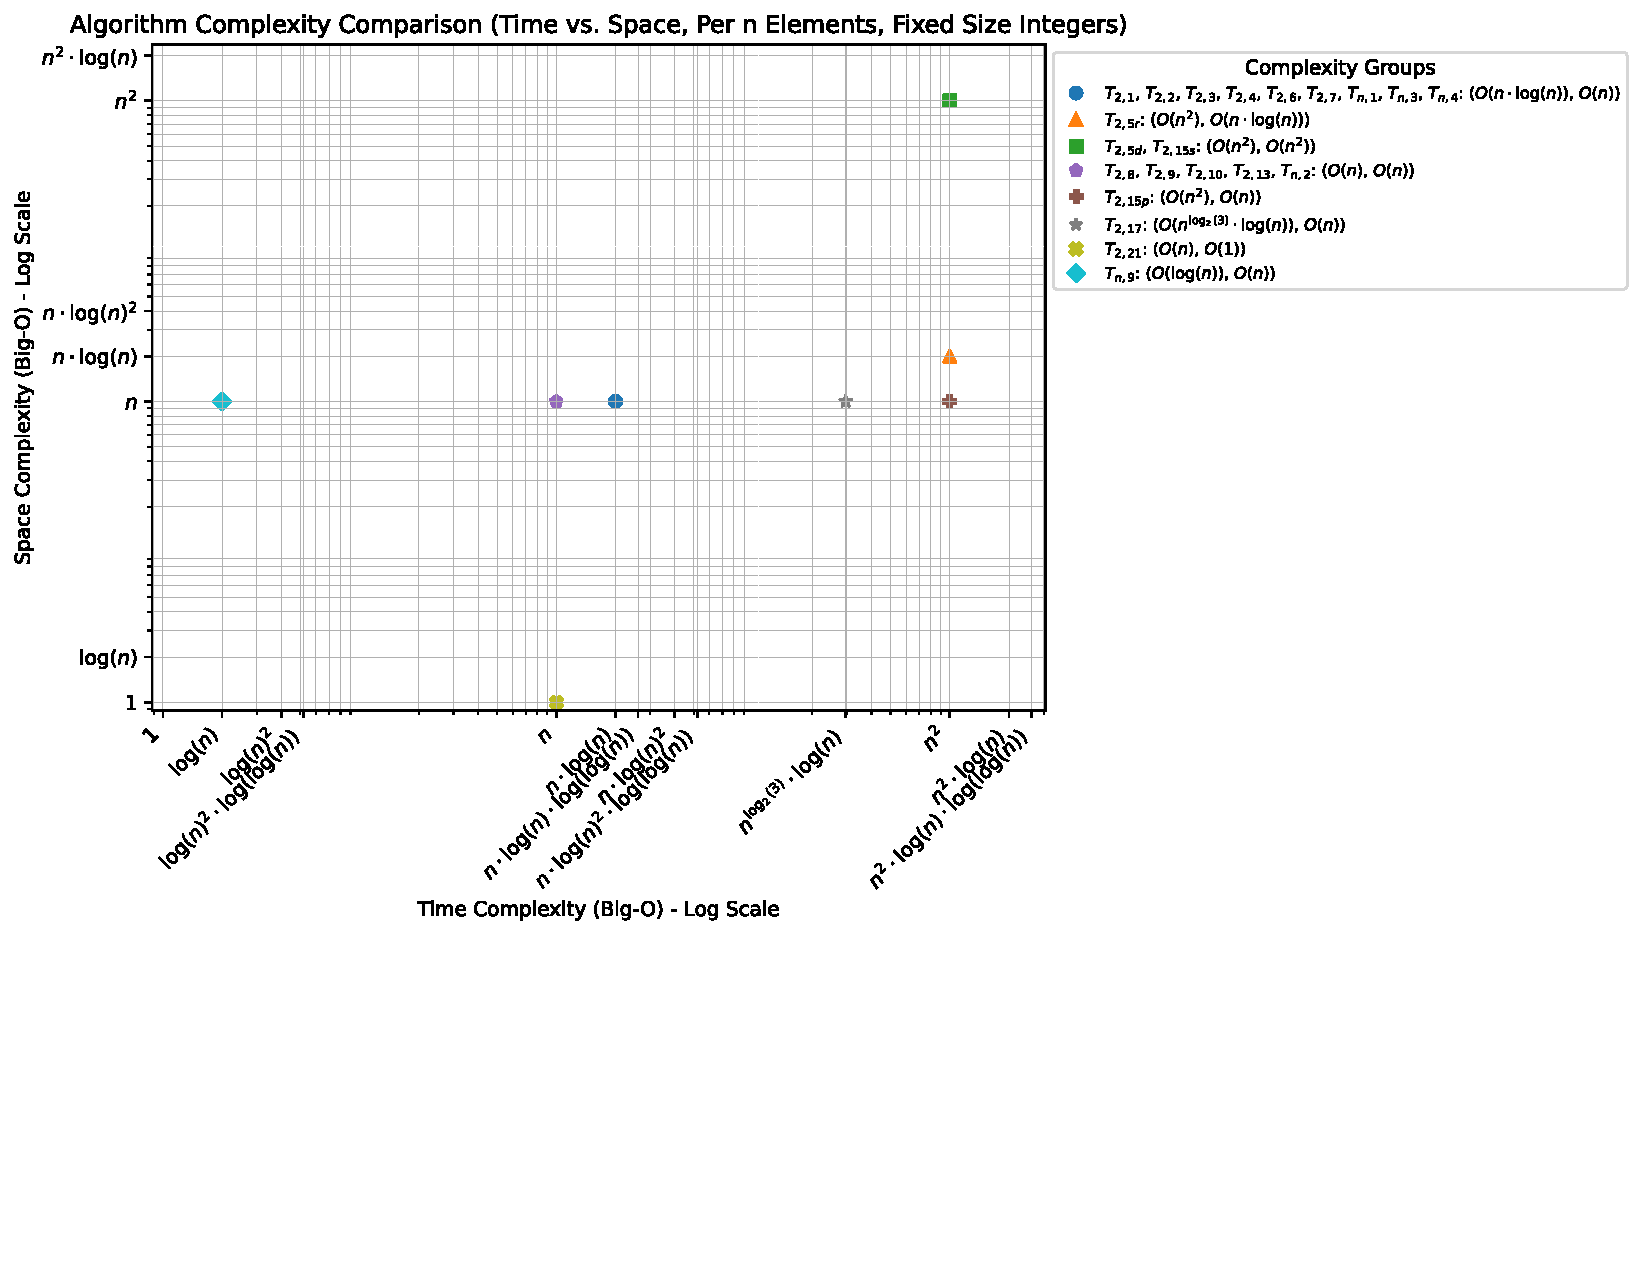
\includegraphics[width=\linewidth, trim=0 0 0 0, clip]{figures/complexity/complexity_comparison_1_0.pdf}
    \label{fig:complexity_1_0}
    \vspace{-25pt}
\end{figure}

\begin{figure}[H]
    \centering
    \vspace{-20pt}
    \caption{Compared Complexity for Arbitrary Size Integers and $n$ Elements.}
    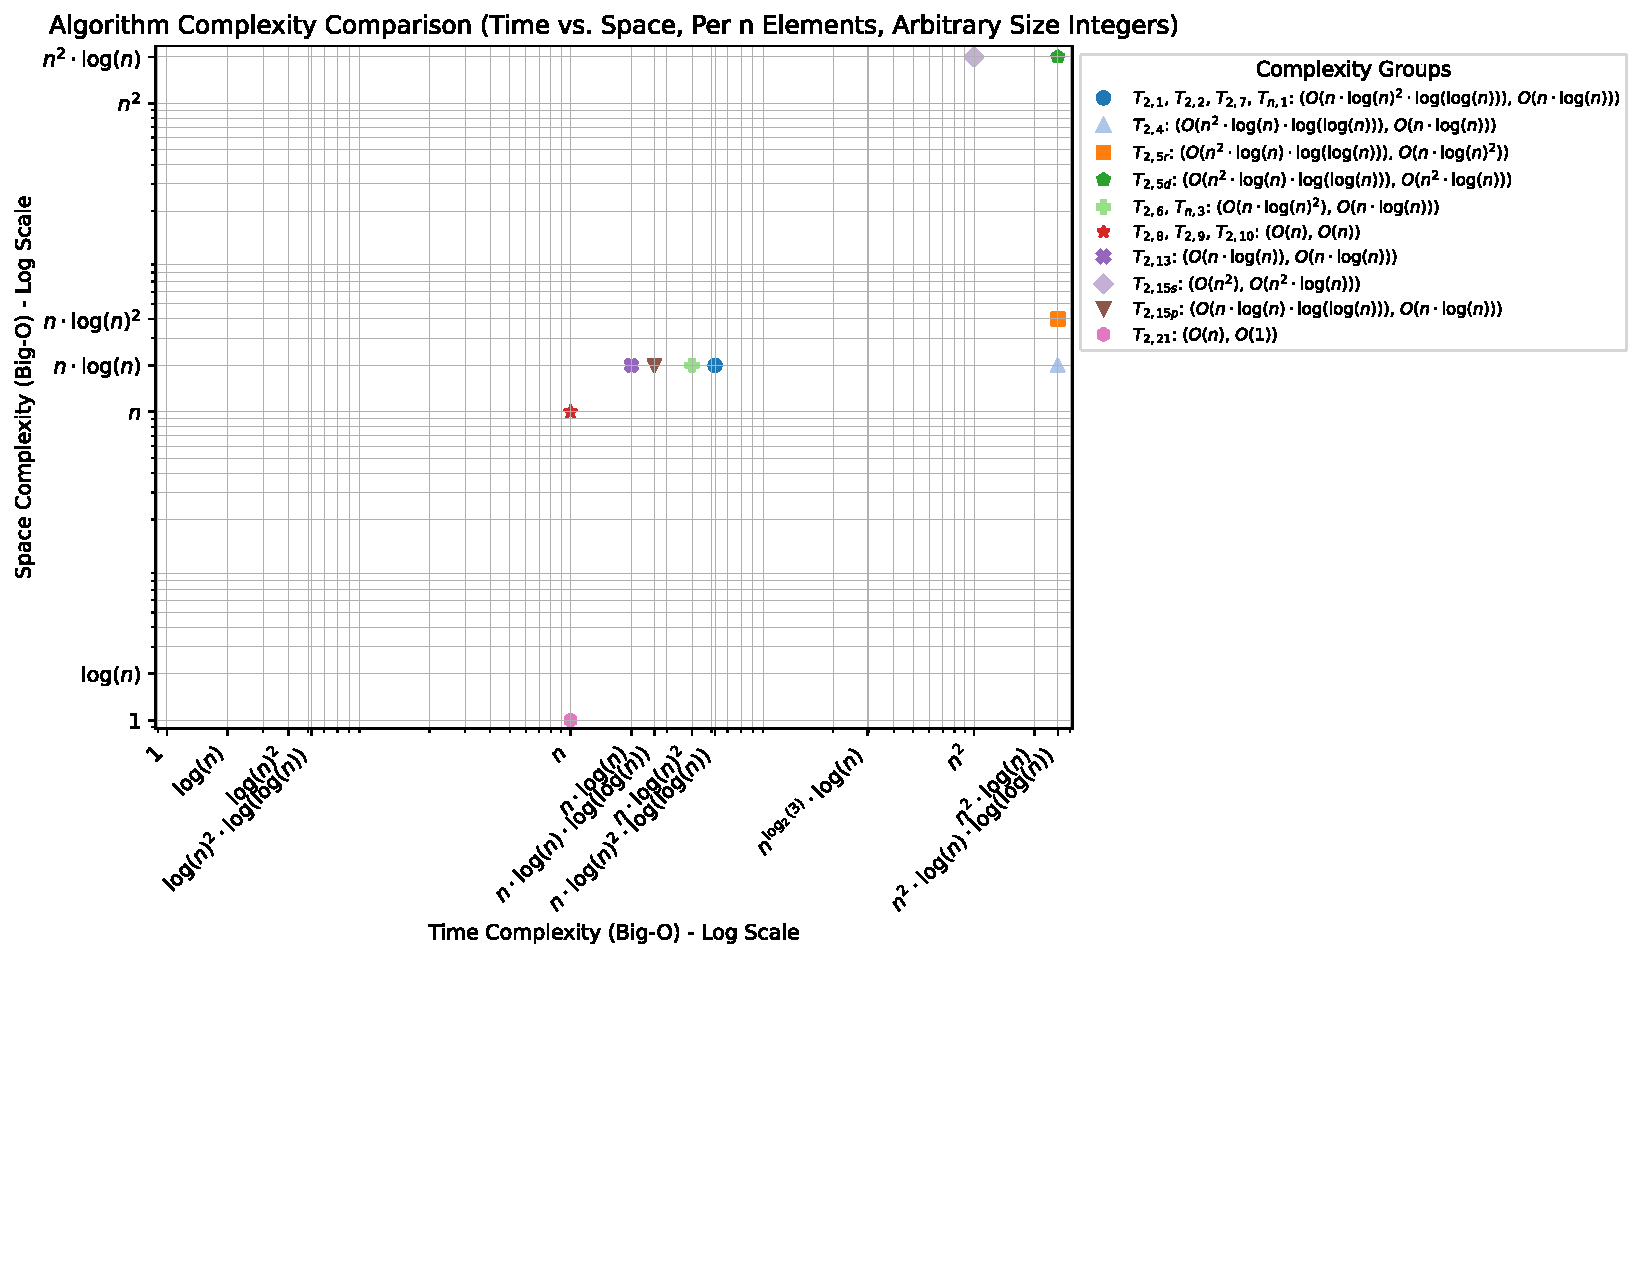
\includegraphics[width=\linewidth, trim=0 0 0 0, clip]{figures/complexity/complexity_comparison_1_1.pdf}
    \label{fig:complexity_1_1}
    \vspace{-25pt}
\end{figure}

\note{These figures are temporary and will be replaced with something prettier when things are finalized}

\section{Appendix 3 --- Complexity of Orig. Definitions}

\setcounter{stddefctr}{1}
\setcounter{extdefctr}{1}

\subsection{Complexity of Original Def. \arabic{stddefctr} --- Parity of Hamming Weight}
\edef\tempLabel{ca:p2_d\arabic{stddefctr}}
\expandafter\label\expandafter\tempLabel

\subsubsection{Time Complexity}

In an idealized case, this definition will simplify to:

\begin{equation}
T_{2,\arabic{stddefctr}}(n) = \left(\sum_{i=0}^{\ceil{\log_2(n + 1)}} \hspace{-8pt} \floor{\dfrac{n}{2^i} \mod{2}} \right) \mod{2}
\end{equation}

This is pretty explicitly $O(\log(n))$ operations. This means that generating the first $n$ entries will take $O(n\log(n))$ operations.

In languages with dynamically sized integers, this can be slightly more complicated. In the above, we perform $\log(n)$ bit shifts, multiplications, moduli, and additions. Since a bit shift is constant time, calculation will be dominated by multiplication, division, and moduli. Each of these take $O(\log(n) \cdot \log(\log(n)))$, where $n$ is the largest number involved. This means that in such languages, we can expect it to take $O(\log(n)^2 \cdot \log(\log(n)))$ operations per element, for $O(n \cdot \log(n)^2 \cdot \log(\log(n)))$ in total.

\renewcommand{\arraystretch}{1.25}
\begin{table}[H]
    \centering
    \caption{Time Complexity Summary of Standard Definition \arabic{stddefctr}}
    \begin{tabular}{|c|c|c|}
        \hline
        & \textbf{Fixed Size} & \textbf{Arbitrary Size} \\
        \hline
        \textbf{Per Element} & $O(\log(n))$ & $O(\log(n)^2 \cdot \log(\log(n)))$ \\
        \hline
        \textbf{In Total} & $O(n \cdot \log(n))$ & $O(n \cdot \log(n)^2 \cdot \log(\log(n)))$ \\
        \hline
    \end{tabular}
    \edef\tempLabel{tab:time_p2_d\arabic{stddefctr}}
     \expandafter\label\expandafter\tempLabel
\end{table}
\renewcommand{\arraystretch}{1}

\subsubsection{Space Complexity}

This is one of the more space-efficient implementations. Each element takes at most the same size as the passed integer. In languages that use Fixed Size integers, that means it will take $O(1)$ space. In languages like Python that use Arbitrary Size integers, it would take $O(\log(n))$ space, where $n$ is the largest element you intend to calculate. If you intend to store all $n$ elements, it will therefore take $O(n)$ or $O(n \cdot \log(n))$ space.

\begin{table}[H]
    \centering
    \caption{Space Complexity Summary of Standard Definition \arabic{stddefctr}}
    \begin{tabular}{|c|c|c|}
        \hline
        & \textbf{Fixed Size} & \textbf{Arbitrary Size} \\
        \hline
        \textbf{Per Element} & $O(1)$ & $O(\log(n))$ \\
        \hline
        \textbf{In Total} & $O(n)$ & $O(n \cdot \log(n))$ \\
        \hline
    \end{tabular}
    \edef\tempLabel{tab:space_p2_d\arabic{stddefctr}}
     \expandafter\label\expandafter\tempLabel
\end{table}

\stepcounter{stddefctr}
\subsection{Complexity of Original Def. \arabic{stddefctr} --- Powers of Negative One}
\edef\tempLabel{ca:p2_d\arabic{stddefctr}}
 \expandafter\label\expandafter\tempLabel

\subsubsection{Time Complexity}

This algorithm is dominated by the time it takes to calculate $p()$, as raising $(-1)$ to a power just requires a number of sign flips. This means we can duplicate the analysis from above.

\begin{table}[H]
    \centering
    \caption{Time Complexity Summary of Standard Definition \arabic{stddefctr}}
    \begin{tabular}{|c|c|c|}
        \hline
        & \textbf{Fixed Size} & \textbf{Arbitrary Size} \\
        \hline
        \textbf{Per Element} & $O(\log(n))$ & $O(\log(n)^2 \cdot \log(\log(n)))$ \\
        \hline
        \textbf{In Total} & $O(n \cdot \log(n))$ & $O(n \cdot \log(n)^2 \cdot \log(\log(n)))$ \\
        \hline
    \end{tabular}
    \edef\tempLabel{tab:time_p2_d\arabic{stddefctr}}
     \expandafter\label\expandafter\tempLabel
\end{table}

\subsubsection{Space Complexity}
\par\noindent\par

\begin{table}[H]
    \centering
    \caption{Space Complexity Summary of Standard Definition \arabic{stddefctr}}
    \begin{tabular}{|c|c|c|}
        \hline
        & \textbf{Fixed Size} & \textbf{Arbitrary Size} \\
        \hline
        \textbf{Per Element} & $O(1)$ & $O(\log(n))$ \\
        \hline
        \textbf{In Total} & $O(n)$ & $O(n \cdot \log(n))$ \\
        \hline
    \end{tabular}
    \edef\tempLabel{tab:space_p2_d\arabic{stddefctr}}
     \expandafter\label\expandafter\tempLabel
\end{table}

\stepcounter{stddefctr}
\subsection{Complexity of Original Definition \arabic{stddefctr} --- Root of Unity}
\edef\tempLabel{ca:p2_d\arabic{stddefctr}}
 \expandafter\label\expandafter\tempLabel

\subsubsection{Time Complexity} ...

\begin{table}[H]
    \centering
    \caption{Time Complexity Summary of Standard Definition \arabic{stddefctr}}
    \begin{tabular}{|c|c|c|}
        \hline
        & \textbf{Fixed Size} & \textbf{Arbitrary Size} \\
        \hline
        \textbf{Per Element} &  &  \\
        \hline
        \textbf{In Total} &  &  \\
        \hline
    \end{tabular}
    \edef\tempLabel{tab:time_p2_d\arabic{stddefctr}}
     \expandafter\label\expandafter\tempLabel
\end{table}

\subsubsection{Space Complexity} ...

\begin{table}[H]
    \centering
    \caption{Space Complexity Summary of Standard Definition \arabic{stddefctr}}
    \begin{tabular}{|c|c|c|}
        \hline
        & \textbf{Fixed Size} & \textbf{Arbitrary Size} \\
        \hline
        \textbf{Per Element} &  &  \\
        \hline
        \textbf{In Total} &  &  \\
        \hline
    \end{tabular}
    \edef\tempLabel{tab:space_p2_d\arabic{stddefctr}}
     \expandafter\label\expandafter\tempLabel
\end{table}

\stepcounter{stddefctr}
\subsection{Complexity of Original Definition \arabic{stddefctr} --- Recursion}
\edef\tempLabel{ca:p2_d\arabic{stddefctr}}
 \expandafter\label\expandafter\tempLabel

\subsubsection{Time Complexity}

At each step in calculation, the value of $n$ passed to the next recursion is halved. This means that it will take $O(\log_2(n))$ recursive steps. Each recursion involves at maximum 2 subtractions and a bit shift. In most languages with Fixed Size integers, this will take constant time. However, in languages with Arbitrary Size integers these subtractions will typically take $O(\log(n))$, where $n$ is the largest integer in the operation. This means we can expect it to take $O(\log(n)^2$ operations.

\renewcommand{\arraystretch}{1.25}
\begin{table}[H]
    \centering
    \caption{Time Complexity Summary of Standard Definition \arabic{stddefctr}}
    \begin{tabular}{|c|c|c|}
        \hline
        & \textbf{Fixed Size} & \textbf{Arbitrary Size} \\
        \hline
        \textbf{Per Element} & $O(\log(n))$ & $O(\log(n)^2)$ \\
        \hline
        \textbf{In Total} & $O(n \cdot \log(n))$ & $O(n \cdot \log(n)^2)$ \\
        \hline
    \end{tabular}
    \edef\tempLabel{tab:time_p2_d\arabic{stddefctr}}
     \expandafter\label\expandafter\tempLabel
\end{table}
\renewcommand{\arraystretch}{1}

\subsubsection{Space Complexity}

This is one of the more space-efficient implementations. Each element takes at most the same size as the passed integer. In languages that use Fixed Size integers, that means it will take $O(1)$ space. In languages like Python that use Arbitrary Size integers, it would take $O(\log(n))$ space, where $n$ is the largest element you intend to calculate. If you intend to store all $n$ elements, it will therefore take $O(n)$ or $O(n \cdot \log(n))$ space.

\begin{table}[H]
    \centering
    \caption{Space Complexity Summary of Standard Definition \arabic{stddefctr}}
    \begin{tabular}{|c|c|c|}
        \hline
        & \textbf{Fixed Size} & \textbf{Arbitrary Size} \\
        \hline
        \textbf{Per Element} & $O(1)$ & $O(\log(n))$ \\
        \hline
        \textbf{In Total} & $O(n)$ & $O(n \cdot \log(n))$ \\
        \hline
    \end{tabular}
    \edef\tempLabel{tab:space_p2_d\arabic{stddefctr}}
     \expandafter\label\expandafter\tempLabel
\end{table}

\stepcounter{stddefctr}
\subsection{Complexity of Original Def. \arabic{stddefctr} --- Floor-Ceiling Difference}
\edef\tempLabel{ca:p2_d\arabic{stddefctr}}
 \expandafter\label\expandafter\tempLabel

\subsubsection{Time Complexity}

\note{memoization doesn't seem to help in the worst case of $1\ldots1_2$, so you should still end up calculating the value of $b()$ for every positive number less than $n$}

\renewcommand{\arraystretch}{1.25}
\begin{table}[H]
    \centering
    \caption{Time Complexity Summary of Standard Definition \arabic{stddefctr}}
    \begin{tabular}{|c|c|c|}
        \hline
        & \textbf{Fixed Size} & \textbf{Arbitrary Size} \\
        \hline
        \textbf{Per Element} & $O(n)$ & $O(n \cdot \log(n) \cdot \log(\log(n)))$ \\
        \hline
        \textbf{In Total} & $O\left(n^2\right)$ & $O\left(n^2 \cdot \log(n) \cdot \log(\log(n))\right)$ \\
        \hline
    \end{tabular}
    \edef\tempLabel{tab:time_p2_d\arabic{stddefctr}}
     \expandafter\label\expandafter\tempLabel
\end{table}

\subsubsection{Space Complexity}

There are two ways to implement this algorithm in terms of space complexity. They both have equal worst-case time complexity. The first is to take the recursive approach, and the second is to use dynamic programming.

In a recursive approach, you will end up descending $O(\log(n))$ stack frames, each of which will contain at minimum 1 integer. In the dynamic approach, you will keep a table of all the values of $b()$ from $0$ through $n$. The biggest difference between these approaches is that in the recursive approach you may need to repeat calculations.

\begin{table}[H]
    \centering
    \caption{Space Complexity Summary of Standard Definition \arabic{stddefctr}}
    \begin{tabular}{|cc|c|c|}
        \hline
        & & \textbf{Fixed Size} & \textbf{Arbitrary Size} \\
        \hline
        \multirow{2}{*}{\textbf{Recursive}} \hspace{-5pt} & \textbf{Per Element} & $O(\log(n))$ & $O(n \cdot \log(n))$ \\
        \cline{2-4}
        & \textbf{In Total} & $O(n \cdot \log(n))$ & $O\left(n^2 \cdot \log(n)\right)$ \\
        \hline
        \multirow{2}{*}{\textbf{Dynamic}} \hspace{-5pt} & \textbf{Per Element} & $O(n)$ & $O(n \cdot \log(n))$ \\
        \cline{2-4}
        & \textbf{In Total} & $O\left(n^2\right)$ & $O\left(n^2 \cdot \log(n)\right)$ \\
        \hline
    \end{tabular}
    \edef\tempLabel{tab:space_p2_d\arabic{stddefctr}}
     \expandafter\label\expandafter\tempLabel
\end{table}
\renewcommand{\arraystretch}{1}

\stepcounter{stddefctr}
\subsection{Complexity of Original Def. \arabic{stddefctr} --- Highest Bit Difference}
\edef\tempLabel{ca:p2_d\arabic{stddefctr}}
 \expandafter\label\expandafter\tempLabel

\subsubsection{Time Complexity}

\note{Since this algorithm works sequentially, and cannot perform computation of an arbitrary element without recursing to the base case, the time is equal on a per-element and in-total basis}

\renewcommand{\arraystretch}{1.25}
\begin{table}[H]
    \centering
    \caption{Time Complexity Summary of Standard Definition \arabic{stddefctr}}
    \begin{tabular}{|c|c|c|}
        \hline
        & \textbf{Fixed Size} & \textbf{Arbitrary Size} \\
        \hline
        \textbf{Per Element} & $O(n \cdot \log(n))$ & $O\left(n \cdot \log(n)^2\right)$ \\
        \hline
        \textbf{In Total} & $O(n \cdot \log(n))$ & $O\left(n \cdot \log(n)^2\right)$ \\
        \hline
    \end{tabular}
    \edef\tempLabel{tab:time_p2_d\arabic{stddefctr}}
     \expandafter\label\expandafter\tempLabel
\end{table}
\renewcommand{\arraystretch}{1}

\subsubsection{Space Complexity} \par\noindent\par

\begin{table}[H]
    \centering
    \caption{Space Complexity Summary of Standard Definition \arabic{stddefctr}}
    \begin{tabular}{|c|c|c|}
        \hline
        & \textbf{Fixed Size} & \textbf{Arbitrary Size} \\
        \hline
        \textbf{Per Element} & $O(1)$ & $O(\log(n))$ \\
        \hline
        \textbf{In Total} & $O(n)$ & $O(n \cdot \log(n))$ \\
        \hline
    \end{tabular}
    \edef\tempLabel{tab:space_p2_d\arabic{stddefctr}}
     \expandafter\label\expandafter\tempLabel
\end{table}

\stepcounter{stddefctr}
\subsection{Complexity of Orig. Def. \arabic{stddefctr} --- Hamming Weight Compl.}
\edef\tempLabel{ca:p2_d\arabic{stddefctr}}
 \expandafter\label\expandafter\tempLabel

\subsubsection{Time Complexity} Like in $T_{2,2}$, this definition is dominated by the calculation of $p()$ inside of $\overline{p}()$. This means that we can duplicate the analysis there.

\renewcommand{\arraystretch}{1.25}
\begin{table}[H]
    \centering
    \caption{Time Complexity Summary of Standard Definition \arabic{stddefctr}}
    \begin{tabular}{|c|c|c|}
        \hline
        & \textbf{Fixed Size} & \textbf{Arbitrary Size} \\
        \hline
        \textbf{Per Element} & $O(\log(n))$ & $O(\log(n)^2 \cdot \log(\log(n)))$ \\
        \hline
        \textbf{In Total} & $O(n \cdot \log(n))$ & $O(n \cdot \log(n)^2 \cdot \log(\log(n)))$ \\
        \hline
    \end{tabular}
    \edef\tempLabel{tab:time_p2_d\arabic{stddefctr}}
     \expandafter\label\expandafter\tempLabel
\end{table}
\renewcommand{\arraystretch}{1}

\subsubsection{Space Complexity} \par\noindent\par

\begin{table}[H]
    \centering
    \caption{Space Complexity Summary of Standard Definition \arabic{stddefctr}}
    \begin{tabular}{|c|c|c|}
        \hline
        & \textbf{Fixed Size} & \textbf{Arbitrary Size} \\
        \hline
        \textbf{Per Element} & $O(1)$ & $O(\log(n))$ \\
        \hline
        \textbf{In Total} & $O(n)$ & $O(n \cdot \log(n))$ \\
        \hline
    \end{tabular}
    \edef\tempLabel{tab:space_p2_d\arabic{stddefctr}}
     \expandafter\label\expandafter\tempLabel
\end{table}

\stepcounter{stddefctr}
\subsection{Complexity of Original Definition \arabic{stddefctr} --- Invert and Extend}
\edef\tempLabel{ca:p2_d\arabic{stddefctr}}
 \expandafter\label\expandafter\tempLabel

\subsubsection{Time Complexity} ...

\begin{table}[H]
    \centering
    \caption{Time Complexity Summary of Standard Definition \arabic{stddefctr}}
    \begin{tabular}{|c|c|c|}
        \hline
        & \textbf{Fixed Size} & \textbf{Arbitrary Size} \\
        \hline
        \textbf{Per Element} &  &  \\
        \hline
        \textbf{In Total} &  &  \\
        \hline
    \end{tabular}
    \edef\tempLabel{tab:time_p2_d\arabic{stddefctr}}
     \expandafter\label\expandafter\tempLabel
\end{table}

\subsubsection{Space Complexity} ...

\begin{table}[H]
    \centering
    \caption{Space Complexity Summary of Standard Definition \arabic{stddefctr}}
    \begin{tabular}{|c|c|c|}
        \hline
        & \textbf{Fixed Size} & \textbf{Arbitrary Size} \\
        \hline
        \textbf{Per Element} &  &  \\
        \hline
        \textbf{In Total} &  &  \\
        \hline
    \end{tabular}
    \edef\tempLabel{tab:space_p2_d\arabic{stddefctr}}
     \expandafter\label\expandafter\tempLabel
\end{table}

\stepcounter{stddefctr}
\subsection{Complexity of Original Def. \arabic{stddefctr} --- Substitute and Flatten}
\edef\tempLabel{ca:p2_d\arabic{stddefctr}}
 \expandafter\label\expandafter\tempLabel

\subsubsection{Time Complexity} ...

\begin{table}[H]
    \centering
    \caption{Time Complexity Summary of Standard Definition \arabic{stddefctr}}
    \begin{tabular}{|c|c|c|}
        \hline
        & \textbf{Fixed Size} & \textbf{Arbitrary Size} \\
        \hline
        \textbf{Per Element} &  &  \\
        \hline
        \textbf{In Total} &  &  \\
        \hline
    \end{tabular}
    \edef\tempLabel{tab:time_p2_d\arabic{stddefctr}}
     \expandafter\label\expandafter\tempLabel
\end{table}

\subsubsection{Space Complexity} ...

\begin{table}[H]
    \centering
    \caption{Space Complexity Summary of Standard Definition \arabic{stddefctr}}
    \begin{tabular}{|c|c|c|}
        \hline
        & \textbf{Fixed Size} & \textbf{Arbitrary Size} \\
        \hline
        \textbf{Per Element} &  &  \\
        \hline
        \textbf{In Total} &  &  \\
        \hline
    \end{tabular}
    \edef\tempLabel{tab:space_p2_d\arabic{stddefctr}}
     \expandafter\label\expandafter\tempLabel
\end{table}

\stepcounter{stddefctr}
\subsection{Complexity of Original Definition \arabic{stddefctr} --- Recursive Rotation}
\edef\tempLabel{ca:p2_d\arabic{stddefctr}}
 \expandafter\label\expandafter\tempLabel

\subsubsection{Time Complexity} ...

\begin{table}[H]
    \centering
    \caption{Time Complexity Summary of Standard Definition \arabic{stddefctr}}
    \begin{tabular}{|c|c|c|}
        \hline
        & \textbf{Fixed Size} & \textbf{Arbitrary Size} \\
        \hline
        \textbf{Per Element} &  &  \\
        \hline
        \textbf{In Total} &  &  \\
        \hline
    \end{tabular}
    \edef\tempLabel{tab:time_p2_d\arabic{stddefctr}}
     \expandafter\label\expandafter\tempLabel
\end{table}

\subsubsection{Space Complexity} ...

\begin{table}[H]
    \centering
    \caption{Space Complexity Summary of Standard Definition \arabic{stddefctr}}
    \begin{tabular}{|c|c|c|}
        \hline
        & \textbf{Fixed Size} & \textbf{Arbitrary Size} \\
        \hline
        \textbf{Per Element} &  &  \\
        \hline
        \textbf{In Total} &  &  \\
        \hline
    \end{tabular}
    \edef\tempLabel{tab:space_p2_d\arabic{stddefctr}}
     \expandafter\label\expandafter\tempLabel
\end{table}

\stepcounter{stddefctr}
\subsection{Complexity of Orig. Def. \arabic{stddefctr} --- Odious Number Derivation}
\edef\tempLabel{ca:p2_d\arabic{stddefctr}}
 \expandafter\label\expandafter\tempLabel

\subsubsection{Time Complexity} ...

\begin{table}[H]
    \centering
    \caption{Time Complexity Summary of Standard Definition \arabic{stddefctr}}
    \begin{tabular}{|c|c|c|}
        \hline
        & \textbf{Fixed Size} & \textbf{Arbitrary Size} \\
        \hline
        \textbf{Per Element} &  &  \\
        \hline
        \textbf{In Total} &  &  \\
        \hline
    \end{tabular}
    \edef\tempLabel{tab:time_p2_d\arabic{stddefctr}}
     \expandafter\label\expandafter\tempLabel
\end{table}

\subsubsection{Space Complexity} ...

\begin{table}[H]
    \centering
    \caption{Space Complexity Summary of Standard Definition \arabic{stddefctr}}
    \begin{tabular}{|c|c|c|}
        \hline
        & \textbf{Fixed Size} & \textbf{Arbitrary Size} \\
        \hline
        \textbf{Per Element} &  &  \\
        \hline
        \textbf{In Total} &  &  \\
        \hline
    \end{tabular}
    \edef\tempLabel{tab:space_p2_d\arabic{stddefctr}}
     \expandafter\label\expandafter\tempLabel
\end{table}

\stepcounter{stddefctr}
\subsection{Complexity of Orig. Def. \arabic{stddefctr} --- Evil Numbers Derivation 1}
\edef\tempLabel{ca:p2_d\arabic{stddefctr}}
 \expandafter\label\expandafter\tempLabel

\subsubsection{Time Complexity} ...

\begin{table}[H]
    \centering
    \caption{Time Complexity Summary of Standard Definition \arabic{stddefctr}}
    \begin{tabular}{|c|c|c|}
        \hline
        & \textbf{Fixed Size} & \textbf{Arbitrary Size} \\
        \hline
        \textbf{Per Element} &  &  \\
        \hline
        \textbf{In Total} &  &  \\
        \hline
    \end{tabular}
    \edef\tempLabel{tab:time_p2_d\arabic{stddefctr}}
     \expandafter\label\expandafter\tempLabel
\end{table}

\subsubsection{Space Complexity} ...

\begin{table}[H]
    \centering
    \caption{Space Complexity Summary of Standard Definition \arabic{stddefctr}}
    \begin{tabular}{|c|c|c|}
        \hline
        & \textbf{Fixed Size} & \textbf{Arbitrary Size} \\
        \hline
        \textbf{Per Element} &  &  \\
        \hline
        \textbf{In Total} &  &  \\
        \hline
    \end{tabular}
    \edef\tempLabel{tab:space_p2_d\arabic{stddefctr}}
     \expandafter\label\expandafter\tempLabel
\end{table}

\stepcounter{stddefctr}
\subsection{Complexity of Orig. Def. \arabic{stddefctr} --- Evil Nums. Derivation 2}
\edef\tempLabel{ca:p2_d\arabic{stddefctr}}
 \expandafter\label\expandafter\tempLabel

\subsubsection{Time Complexity} ...

\begin{table}[H]
    \centering
    \caption{Time Complexity Summary of Standard Definition \arabic{stddefctr}}
    \begin{tabular}{|c|c|c|}
        \hline
        & \textbf{Fixed Size} & \textbf{Arbitrary Size} \\
        \hline
        \textbf{Per Element} &  &  \\
        \hline
        \textbf{In Total} &  &  \\
        \hline
    \end{tabular}
    \edef\tempLabel{tab:time_p2_d\arabic{stddefctr}}
     \expandafter\label\expandafter\tempLabel
\end{table}

\subsubsection{Space Complexity} ...

\begin{table}[H]
    \centering
    \caption{Space Complexity Summary of Standard Definition \arabic{stddefctr}}
    \begin{tabular}{|c|c|c|}
        \hline
        & \textbf{Fixed Size} & \textbf{Arbitrary Size} \\
        \hline
        \textbf{Per Element} &  &  \\
        \hline
        \textbf{In Total} &  &  \\
        \hline
    \end{tabular}
    \edef\tempLabel{tab:space_p2_d\arabic{stddefctr}}
     \expandafter\label\expandafter\tempLabel
\end{table}

\stepcounter{stddefctr}
\subsection{Complexity of Orig. Def. \arabic{stddefctr} --- Odious \& Evil Derivation}
\edef\tempLabel{ca:p2_d\arabic{stddefctr}}
 \expandafter\label\expandafter\tempLabel

\subsubsection{Time Complexity} ...

\begin{table}[H]
    \centering
    \caption{Time Complexity Summary of Standard Definition \arabic{stddefctr}}
    \begin{tabular}{|c|c|c|}
        \hline
        & \textbf{Fixed Size} & \textbf{Arbitrary Size} \\
        \hline
        \textbf{Per Element} &  &  \\
        \hline
        \textbf{In Total} &  &  \\
        \hline
    \end{tabular}
    \edef\tempLabel{tab:time_p2_d\arabic{stddefctr}}
     \expandafter\label\expandafter\tempLabel
\end{table}

\subsubsection{Space Complexity} ...

\begin{table}[H]
    \centering
    \caption{Space Complexity Summary of Standard Definition \arabic{stddefctr}}
    \begin{tabular}{|c|c|c|}
        \hline
        & \textbf{Fixed Size} & \textbf{Arbitrary Size} \\
        \hline
        \textbf{Per Element} &  &  \\
        \hline
        \textbf{In Total} &  &  \\
        \hline
    \end{tabular}
    \edef\tempLabel{tab:space_p2_d\arabic{stddefctr}}
     \expandafter\label\expandafter\tempLabel
\end{table}

\stepcounter{stddefctr}
\subsection{Complexity of Orig. Def. \arabic{stddefctr} --- Gould's Seq. Derivation}
\edef\tempLabel{ca:p2_d\arabic{stddefctr}}
 \expandafter\label\expandafter\tempLabel

\subsubsection{Time Complexity}

There are two ways one could reasonably calculate this. The first is by building each row of Pascal's Triangle iteratively. This allows you to avoid multiplication whenever possible, and lets you apply a bitmask or modulus operation to take the parity of each entry. The downside is that this version is not parallelizable. Using the bit mask approach, this means that each entry will take $O(n)$ time.

The other is to take advantage of the relation $\binom{n}{k} = \binom{n}{k-1} \cdot \dfrac{n - (k - 1)}{k}$. This allows you to calculate each row independently, using $\tfrac{n}{2}$ moduli, multiplications, and divisions. This means that each entry will take $O(n)$ operations, each of which take $O(\log(n) \cdot \log(\log(n)))$ if with arbitrary sized integers, totaling $O(n)$ or $O(n \cdot \log(n) \cdot \log(\log(n)))$.

\renewcommand{\arraystretch}{1.25}
\begin{table}[H]
    \centering
    \caption{Time Complexity Summary of Standard Definition \arabic{stddefctr}}
    \begin{tabular}{|cc|c|c|}
        \hline
        & & \textbf{Fixed Size} & \textbf{Arbitrary Size} \\
        \hline
        \multirow{2}{*}{\textbf{Serial}} \hspace{-5pt} & \textbf{Per Element} & $O(n)$ & $O(n)$ \\
        \cline{2-4}
        & \textbf{In Total} & $O\left(n^2\right)$ & $O\left(n^2\right)$ \\
        \hline
        \multirow{2}{*}{\textbf{Parallel}} \hspace{-5pt} & \textbf{Per Element} & $O(n) $ & $O(n \cdot \log(n) \cdot \log(\log(n)))$ \\
        \cline{2-4}
        & \textbf{In Total} & $O\left(n^2\right) $ & $O\left(n^2 \cdot \log(n) \cdot \log(\log(n))\right)$ \\
        \hline
    \end{tabular}
    \edef\tempLabel{tab:time_p2_d\arabic{stddefctr}}
     \expandafter\label\expandafter\tempLabel
\end{table}


\subsubsection{Space Complexity} \par\noindent\par

\begin{table}[H]
    \centering
    \caption{Space Complexity Summary of Standard Definition \arabic{stddefctr}}
    \begin{tabular}{|cc|c|c|}
        \hline
        & & \textbf{Fixed Size} & \textbf{Arbitrary Size} \\
        \hline
        \multirow{2}{*}{\textbf{Serial}} \hspace{-5pt} & \textbf{Per Element} & $O(n)$ & $O\left(n \cdot \log(n)\right)$ \\
        \cline{2-4}
        & \textbf{In Total} & $O\left(n^2\right)$ & $O\left(n^2 \cdot \log(n)\right)$ \\
        \hline
        \multirow{2}{*}{\textbf{Parallel}} \hspace{-5pt} & \textbf{Per Element} & $O(1)$ & $O\left(\log(n)\right)$ \\
        \cline{2-4}
        & \textbf{In Total} & $O(n)$ & $O\left(n \cdot \log(n)^2\right)$ \\
        \hline
    \end{tabular}
    \edef\tempLabel{tab:space_p2_d\arabic{stddefctr}}
     \expandafter\label\expandafter\tempLabel
\end{table}
\renewcommand{\arraystretch}{1}

\stepcounter{stddefctr}
\subsection{Complexity of Orig. Def. \arabic{stddefctr} --- Derivation from Blue Code}
\edef\tempLabel{ca:p2_d\arabic{stddefctr}}
 \expandafter\label\expandafter\tempLabel

\subsubsection{Time Complexity} ...

\begin{table}[H]
    \centering
    \caption{Time Complexity Summary of Standard Definition \arabic{stddefctr}}
    \begin{tabular}{|c|c|c|}
        \hline
        & \textbf{Fixed Size} & \textbf{Arbitrary Size} \\
        \hline
        \textbf{Per Element} &  &  \\
        \hline
        \textbf{In Total} &  &  \\
        \hline
    \end{tabular}
    \edef\tempLabel{tab:time_p2_d\arabic{stddefctr}}
     \expandafter\label\expandafter\tempLabel
\end{table}

\subsubsection{Space Complexity} ...

\begin{table}[H]
    \centering
    \caption{Space Complexity Summary of Standard Definition \arabic{stddefctr}}
    \begin{tabular}{|c|c|c|}
        \hline
        & \textbf{Fixed Size} & \textbf{Arbitrary Size} \\
        \hline
        \textbf{Per Element} &  &  \\
        \hline
        \textbf{In Total} &  &  \\
        \hline
    \end{tabular}
    \edef\tempLabel{tab:space_p2_d\arabic{stddefctr}}
     \expandafter\label\expandafter\tempLabel
\end{table}

\stepcounter{stddefctr}
\subsection{Complexity of Original Def. \arabic{stddefctr} --- Generating Function 1}
\edef\tempLabel{ca:p2_d\arabic{stddefctr}}
 \expandafter\label\expandafter\tempLabel

\subsubsection{Time Complexity}

\note{Time complexity of multiplying polynomials via Karatsuba method is $O(n^{\log_2(3)})$. I think this means that, since we need to apply it $\log_2(n)$ times to get $n$ terms, the overall complexity is $O(n^{\log_2(3)} \cdot \log(n))$}

\renewcommand{\arraystretch}{1.25}
\begin{table}[H]
    \centering
    \caption{Time Complexity Summary of Standard Definition \arabic{stddefctr}}
    \begin{tabular}{|c|c|c|}
        \hline
        & \textbf{Fixed Size} & \textbf{Arbitrary Size} \\
        \hline
        \textbf{Per Element} & $O\left(n^{\log_2(3)} \cdot \log(n)\right)?$ &  \\
        \hline
        \textbf{In Total} & $O\left(n^{\log_2(3)} \cdot \log(n)\right)$ &  \\
        \hline
    \end{tabular}
    \edef\tempLabel{tab:time_p2_d\arabic{stddefctr}}
     \expandafter\label\expandafter\tempLabel
\end{table}
\renewcommand{\arraystretch}{1}

\subsubsection{Space Complexity} ...

\begin{table}[H]
    \centering
    \caption{Space Complexity Summary of Standard Definition \arabic{stddefctr}}
    \begin{tabular}{|c|c|c|}
        \hline
        & \textbf{Fixed Size} & \textbf{Arbitrary Size} \\
        \hline
        \textbf{Per Element} & $O(n)?$ & $O(n\log(n))?$ \\
        \hline
        \textbf{In Total} & $O(n)?$ & $O(n\log(n))?$ \\
        \hline
    \end{tabular}
    \edef\tempLabel{tab:space_p2_d\arabic{stddefctr}}
     \expandafter\label\expandafter\tempLabel
\end{table}


\stepcounter{stddefctr}
\subsection{Complexity of Original Def. \arabic{stddefctr} --- Generating Function 2}
\edef\tempLabel{ca:p2_d\arabic{stddefctr}}
 \expandafter\label\expandafter\tempLabel

\subsubsection{Time Complexity} ...

\renewcommand{\arraystretch}{1.25}
\begin{table}[H]
    \centering
    \caption{Time Complexity Summary of Standard Definition \arabic{stddefctr}}
    \begin{tabular}{|c|c|c|}
        \hline
        & \textbf{Fixed Size} & \textbf{Arbitrary Size} \\
        \hline
        \textbf{Per Element} &  &  \\
        \hline
        \textbf{In Total} &  &  \\
        \hline
    \end{tabular}
    \edef\tempLabel{tab:time_p2_d\arabic{stddefctr}}
     \expandafter\label\expandafter\tempLabel
\end{table}
\renewcommand{\arraystretch}{1}

\subsubsection{Space Complexity} ...

\begin{table}[H]
    \centering
    \caption{Space Complexity Summary of Standard Definition \arabic{stddefctr}}
    \begin{tabular}{|c|c|c|}
        \hline
        & \textbf{Fixed Size} & \textbf{Arbitrary Size} \\
        \hline
        \textbf{Per Element} &  &  \\
        \hline
        \textbf{In Total} &  &  \\
        \hline
    \end{tabular}
    \edef\tempLabel{tab:space_p2_d\arabic{stddefctr}}
     \expandafter\label\expandafter\tempLabel
\end{table}


\stepcounter{stddefctr}
\subsection{Complexity of Original Def. \arabic{stddefctr} --- Hypergeometry}
\edef\tempLabel{ca:p2_d\arabic{stddefctr}}
 \expandafter\label\expandafter\tempLabel

\subsubsection{Time Complexity} ...

\renewcommand{\arraystretch}{1.25}
\begin{table}[H]
    \centering
    \caption{Time Complexity Summary of Standard Definition \arabic{stddefctr}}
    \begin{tabular}{|c|c|c|}
        \hline
        & \textbf{Fixed Size} & \textbf{Arbitrary Size} \\
        \hline
        \textbf{Per Element} &  &  \\
        \hline
        \textbf{In Total} &  &  \\
        \hline
    \end{tabular}
    \edef\tempLabel{tab:time_p2_d\arabic{stddefctr}}
     \expandafter\label\expandafter\tempLabel
\end{table}
\renewcommand{\arraystretch}{1}

\subsubsection{Space Complexity} ...

\begin{table}[H]
    \centering
    \caption{Space Complexity Summary of Standard Definition \arabic{stddefctr}}
    \begin{tabular}{|c|c|c|}
        \hline
        & \textbf{Fixed Size} & \textbf{Arbitrary Size} \\
        \hline
        \textbf{Per Element} &  &  \\
        \hline
        \textbf{In Total} &  &  \\
        \hline
    \end{tabular}
    \edef\tempLabel{tab:space_p2_d\arabic{stddefctr}}
     \expandafter\label\expandafter\tempLabel
\end{table}


\stepcounter{stddefctr}
\subsection{Complexity of Original Def. \arabic{stddefctr} --- Cellular Automaton}
\edef\tempLabel{ca:p2_d\arabic{stddefctr}}
 \expandafter\label\expandafter\tempLabel

\subsubsection{Time Complexity} ...

\renewcommand{\arraystretch}{1.25}
\begin{table}[H]
    \centering
    \caption{Time Complexity Summary of Standard Definition \arabic{stddefctr}}
    \begin{tabular}{|c|c|c|}
        \hline
        & \textbf{Fixed Size} & \textbf{Arbitrary Size} \\
        \hline
        \textbf{Per Element} &  &  \\
        \hline
        \textbf{In Total} &  &  \\
        \hline
    \end{tabular}
    \edef\tempLabel{tab:time_p2_d\arabic{stddefctr}}
     \expandafter\label\expandafter\tempLabel
\end{table}
\renewcommand{\arraystretch}{1}

\subsubsection{Space Complexity} ...

\begin{table}[H]
    \centering
    \caption{Space Complexity Summary of Standard Definition \arabic{stddefctr}}
    \begin{tabular}{|c|c|c|}
        \hline
        & \textbf{Fixed Size} & \textbf{Arbitrary Size} \\
        \hline
        \textbf{Per Element} &  &  \\
        \hline
        \textbf{In Total} &  &  \\
        \hline
    \end{tabular}
    \edef\tempLabel{tab:space_p2_d\arabic{stddefctr}}
     \expandafter\label\expandafter\tempLabel
\end{table}


\stepcounter{stddefctr}
\subsection{Complexity of Original Def. \arabic{stddefctr} --- Galois Duels}
\edef\tempLabel{ca:p2_d\arabic{stddefctr}}
 \expandafter\label\expandafter\tempLabel

\subsubsection{Time Complexity} ...

\renewcommand{\arraystretch}{1.25}
\begin{table}[H]
    \centering
    \caption{Time Complexity Summary of Standard Definition \arabic{stddefctr}}
    \begin{tabular}{|c|c|c|}
        \hline
        & \textbf{Fixed Size} & \textbf{Arbitrary Size} \\
        \hline
        \textbf{Per Element} &  &  \\
        \hline
        \textbf{In Total} &  &  \\
        \hline
    \end{tabular}
    \edef\tempLabel{tab:time_p2_d\arabic{stddefctr}}
     \expandafter\label\expandafter\tempLabel
\end{table}
\renewcommand{\arraystretch}{1}

\subsubsection{Space Complexity} ...

\begin{table}[H]
    \centering
    \caption{Space Complexity Summary of Standard Definition \arabic{stddefctr}}
    \begin{tabular}{|c|c|c|}
        \hline
        & \textbf{Fixed Size} & \textbf{Arbitrary Size} \\
        \hline
        \textbf{Per Element} &  &  \\
        \hline
        \textbf{In Total} &  &  \\
        \hline
    \end{tabular}
    \edef\tempLabel{tab:space_p2_d\arabic{stddefctr}}
     \expandafter\label\expandafter\tempLabel
\end{table}

\section{Appendix 4 --- Complexity of Ext. Definitions}

\subsection{Complexity of Extension Def. \arabic{extdefctr} --- Modular Digit Sums}
\edef\tempLabel{ca:pn_d\arabic{extdefctr}}
 \expandafter\label\expandafter\tempLabel

In an idealized case, this definition will simplify to:

\begin{equation}
T_{n,\arabic{extdefctr}}(x, s) = \left(\sum_{i=0}^{\ceil{\log_s(x + 1)}} \hspace{-8pt} \floor{\dfrac{x}{s^i} \mod{s}} \right) \mod{s}
\end{equation}

This is pretty explicitly $O(\log(n))$ operations. This means that generating the first $n$ entries will take $O(n\log(n))$ operations.

In languages with dynamically sized integers, this can be slightly more complicated. In the above, we perform $\log(n)$ multiplications, moduli, and additions. Since additions are simpler, calculation will be dominated by multiplication, division, and moduli. Each of these take $O(\log(n) \cdot \log(\log(n)))$, where $n$ is the largest number involved. This means that in such languages, we can expect it to take $O(\log(n)^2 \cdot \log(\log(n)))$ operations per element, for $O(n \cdot \log(n)^2 \cdot \log(\log(n)))$ in total.

\renewcommand{\arraystretch}{1.25}
\begin{table}[H]
    \centering
    \caption{Time Complexity Summary of Extended Definition \arabic{extdefctr}}
    \begin{tabular}{|c|c|c|}
        \hline
        & \textbf{Fixed Size} & \textbf{Arbitrary Size} \\
        \hline
        \textbf{Per Element} & $O(\log(n))$ & $O(\log(n)^2 \cdot \log(\log(n)))$ \\
        \hline
        \textbf{In Total} & $O(n \cdot \log(n))$ & $O(n \cdot \log(n)^2 \cdot \log(\log(n)))$ \\
        \hline
    \end{tabular}
     \edef\tempLabel{tab:time_pn_d\arabic{extdefctr}}
     \expandafter\label\expandafter\tempLabel
\end{table}
\renewcommand{\arraystretch}{1}

\subsubsection{Space Complexity}

This is one of the more space-efficient implementation. Each element takes at most the same size as the passed integer. In languages that use Fixed Size integers, that means it will take $O(1)$ space. In languages like Python that use Arbitrary Size integers, it would take $O(\log(n))$ space, where $n$ is the largest element you intend to calculate. If you intend to store all $n$ elements, it will therefore take $O(n)$ or $O(n \cdot \log(n))$ space.

\begin{table}[H]
    \centering
    \caption{Space Complexity Summary of Extended Definition \arabic{extdefctr}}
    \begin{tabular}{|c|c|c|}
        \hline
        & \textbf{Fixed Size} & \textbf{Arbitrary Size} \\
        \hline
        \textbf{Per Element} & $O(1)$ & $O(\log(n))$ \\
        \hline
        \textbf{In Total} & $O(n)$ & $O(n \cdot \log(n))$ \\
        \hline
    \end{tabular}
     \edef\tempLabel{tab:space_pn_d\arabic{extdefctr}}
     \expandafter\label\expandafter\tempLabel
\end{table}

\stepcounter{extdefctr}
\subsection{Complexity of Extension Definition \arabic{extdefctr} --- Roots of Unity}
\edef\tempLabel{ca:pn_d\arabic{extdefctr}}
 \expandafter\label\expandafter\tempLabel

\subsubsection{Time Complexity} ...

\begin{table}[H]
    \centering
    \caption{Time Complexity Summary of Extended Definition \arabic{extdefctr}}
    \begin{tabular}{|c|c|c|}
        \hline
        & \textbf{Fixed Size} & \textbf{Arbitrary Size} \\
        \hline
        \textbf{Per Element} &  &  \\
        \hline
        \textbf{In Total} &  &  \\
        \hline
    \end{tabular}
     \edef\tempLabel{tab:time_pn_d\arabic{extdefctr}}
     \expandafter\label\expandafter\tempLabel
\end{table}

\subsubsection{Space Complexity} ...

\begin{table}[H]
    \centering
    \caption{Space Complexity Summary of Extended Definition \arabic{extdefctr}}
    \begin{tabular}{|c|c|c|}
        \hline
        & \textbf{Fixed Size} & \textbf{Arbitrary Size} \\
        \hline
        \textbf{Per Element} &  &  \\
        \hline
        \textbf{In Total} &  &  \\
        \hline
    \end{tabular}
     \edef\tempLabel{tab:space_pn_d\arabic{extdefctr}}
     \expandafter\label\expandafter\tempLabel
\end{table}

\stepcounter{extdefctr}
\subsection{Complexity of Extension Definition \arabic{extdefctr} --- Recursion}
\edef\tempLabel{ca:pn_d\arabic{extdefctr}}
 \expandafter\label\expandafter\tempLabel

\subsubsection{Time Complexity}

At each step in calculation, the value of $n$ passed to the next recursion is divided by $s$ (the selected base). This means that it will take $O(\log_s(n))$ recursive steps. Each recursion involves at maximum 2 subtractions and a bit shift. In most languages with Fixed Size integers, this will take constant time. However, in languages with Arbitrary Size integers these subtractions will typically take $O(\log(n))$, where $n$ is the largest integer in the operation. This means we can expect it to take $O(\log(n)^2$ operations.

\renewcommand{\arraystretch}{1.25}
\begin{table}[H]
    \centering
    \caption{Time Complexity Summary of Extended Definition \arabic{extdefctr}}
    \begin{tabular}{|c|c|c|}
        \hline
        & \textbf{Fixed Size} & \textbf{Arbitrary Size} \\
        \hline
        \textbf{Per Element} & $O(\log(n))$ & $O(\log(n)^2)$ \\
        \hline
        \textbf{In Total} & $O(n \cdot \log(n))$ & $O(n \cdot \log(n)^2)$ \\
        \hline
    \end{tabular}
     \edef\tempLabel{tab:time_pn_d\arabic{extdefctr}}
     \expandafter\label\expandafter\tempLabel
\end{table}
\renewcommand{\arraystretch}{1}

\subsubsection{Space Complexity}

This is one of the more space-efficient implementations. Each element takes at most the same size as the passed integer. In languages that use Fixed Size integers, that means it will take $O(1)$ space. In languages like Python that use Arbitrary Size integers, it would take $O(\log(n))$ space, where $n$ is the largest element you intend to calculate. If you intend to store all $n$ elements, it will therefore take $O(n)$ or $O(n \cdot \log(n))$ space.

\begin{table}[H]
    \centering
    \caption{Space Complexity Summary of Extended Definition \arabic{extdefctr}}
    \begin{tabular}{|c|c|c|}
        \hline
        & \textbf{Fixed Size} & \textbf{Arbitrary Size} \\
        \hline
        \textbf{Per Element} & $O(1)$ & $O(\log(n))$ \\
        \hline
        \textbf{In Total} & $O(n)$ & $O(n \cdot \log(n))$ \\
        \hline
    \end{tabular}
     \edef\tempLabel{tab:space_pn_d\arabic{extdefctr}}
     \expandafter\label\expandafter\tempLabel
\end{table}

\stepcounter{extdefctr}
\subsection{Complexity of Extension Def. \arabic{extdefctr} --- Highest Digit Difference}
\edef\tempLabel{ca:pn_d\arabic{extdefctr}}
 \expandafter\label\expandafter\tempLabel

\subsubsection{Time Complexity} ...

\renewcommand{\arraystretch}{1.25}
\begin{table}[H]
    \centering
    \caption{Time Complexity Summary of Extended Definition \arabic{extdefctr}}
    \begin{tabular}{|c|c|c|}
        \hline
        & \textbf{Fixed Size} & \textbf{Arbitrary Size} \\
        \hline
        \textbf{Per Element} &  &  \\
        \hline
        \textbf{In Total} &  &  \\
        \hline
    \end{tabular}
     \edef\tempLabel{tab:time_pn_d\arabic{extdefctr}}
     \expandafter\label\expandafter\tempLabel
\end{table}
\renewcommand{\arraystretch}{1}

\subsubsection{Space Complexity} ...

\begin{table}[H]
    \centering
    \caption{Space Complexity Summary of Extended Definition \arabic{extdefctr}}
    \begin{tabular}{|c|c|c|}
        \hline
        & \textbf{Fixed Size} & \textbf{Arbitrary Size} \\
        \hline
        \textbf{Per Element} &  &  \\
        \hline
        \textbf{In Total} &  &  \\
        \hline
    \end{tabular}
     \edef\tempLabel{tab:space_pn_d\arabic{extdefctr}}
     \expandafter\label\expandafter\tempLabel
\end{table}

\stepcounter{extdefctr}
\subsection{Complexity of Extension Def. \arabic{extdefctr} --- Increment and Extend}
\edef\tempLabel{ca:pn_d\arabic{extdefctr}}
 \expandafter\label\expandafter\tempLabel

\subsubsection{Time Complexity} ...

\begin{table}[H]
    \centering
    \caption{Time Complexity Summary of Extended Definition \arabic{extdefctr}}
    \begin{tabular}{|c|c|c|}
        \hline
        & \textbf{Fixed Size} & \textbf{Arbitrary Size} \\
        \hline
        \textbf{Per Element} &  &  \\
        \hline
        \textbf{In Total} &  &  \\
        \hline
    \end{tabular}
     \edef\tempLabel{tab:time_pn_d\arabic{extdefctr}}
     \expandafter\label\expandafter\tempLabel
\end{table}

\subsubsection{Space Complexity} ...

\begin{table}[H]
    \centering
    \caption{Space Complexity Summary of Extended Definition \arabic{extdefctr}}
    \begin{tabular}{|c|c|c|}
        \hline
        & \textbf{Fixed Size} & \textbf{Arbitrary Size} \\
        \hline
        \textbf{Per Element} &  &  \\
        \hline
        \textbf{In Total} &  &  \\
        \hline
    \end{tabular}
     \edef\tempLabel{tab:space_pn_d\arabic{extdefctr}}
     \expandafter\label\expandafter\tempLabel
\end{table}

\stepcounter{extdefctr}
\subsection{Complexity of Extension Def. \arabic{extdefctr} --- Substitute and Flatten}
\edef\tempLabel{ca:pn_d\arabic{extdefctr}}
 \expandafter\label\expandafter\tempLabel

\subsubsection{Time Complexity} ...

\begin{table}[H]
    \centering
    \caption{Time Complexity Summary of Extended Definition \arabic{extdefctr}}
    \begin{tabular}{|c|c|c|}
        \hline
        & \textbf{Fixed Size} & \textbf{Arbitrary Size} \\
        \hline
        \textbf{Per Element} &  &  \\
        \hline
        \textbf{In Total} &  &  \\
        \hline
    \end{tabular}
     \edef\tempLabel{tab:time_pn_d\arabic{extdefctr}}
     \expandafter\label\expandafter\tempLabel
\end{table}

\subsubsection{Space Complexity} ...

\begin{table}[H]
    \centering
    \caption{Space Complexity Summary of Extended Definition \arabic{extdefctr}}
    \begin{tabular}{|c|c|c|}
        \hline
        & \textbf{Fixed Size} & \textbf{Arbitrary Size} \\
        \hline
        \textbf{Per Element} &  &  \\
        \hline
        \textbf{In Total} &  &  \\
        \hline
    \end{tabular}
     \edef\tempLabel{tab:space_pn_d\arabic{extdefctr}}
     \expandafter\label\expandafter\tempLabel
\end{table}

\stepcounter{extdefctr}
\subsection{Complexity of Extension Definition \arabic{extdefctr} --- Recursive Rotation}
\edef\tempLabel{ca:pn_d\arabic{extdefctr}}
 \expandafter\label\expandafter\tempLabel

\subsubsection{Time Complexity} ...

\begin{table}[H]
    \centering
    \caption{Time Complexity Summary of Extended Definition \arabic{extdefctr}}
    \begin{tabular}{|c|c|c|}
        \hline
        & \textbf{Fixed Size} & \textbf{Arbitrary Size} \\
        \hline
        \textbf{Per Element} &  &  \\
        \hline
        \textbf{In Total} &  &  \\
        \hline
    \end{tabular}
     \edef\tempLabel{tab:time_pn_d\arabic{extdefctr}}
     \expandafter\label\expandafter\tempLabel
\end{table}

\subsubsection{Space Complexity} ...

\begin{table}[H]
    \centering
    \caption{Space Complexity Summary of Extended Definition \arabic{extdefctr}}
    \begin{tabular}{|c|c|c|}
        \hline
        & \textbf{Fixed Size} & \textbf{Arbitrary Size} \\
        \hline
        \textbf{Per Element} &  &  \\
        \hline
        \textbf{In Total} &  &  \\
        \hline
    \end{tabular}
     \edef\tempLabel{tab:space_pn_d\arabic{extdefctr}}
     \expandafter\label\expandafter\tempLabel
\end{table}

\stepcounter{extdefctr}
\subsection{Complexity of Ext. Def. \arabic{extdefctr} --- Latin Square Constructions}
\edef\tempLabel{ca:pn_d\arabic{extdefctr}}
 \expandafter\label\expandafter\tempLabel

\subsubsection{Time Complexity} ...

\renewcommand{\arraystretch}{1.25}
\begin{table}[H]
    \centering
    \caption{Time Complexity Summary of Extended Definition \arabic{extdefctr}}
    \begin{tabular}{|c|c|c|}
        \hline
        & \textbf{Fixed Size} & \textbf{Arbitrary Size} \\
        \hline
        \textbf{Per Element} &  &  \\
        \hline
        \textbf{In Total} &  &  \\
        \hline
    \end{tabular}
     \edef\tempLabel{tab:time_pn_d\arabic{extdefctr}}
     \expandafter\label\expandafter\tempLabel
\end{table}
\renewcommand{\arraystretch}{1}

\subsubsection{Space Complexity} ...

\begin{table}[H]
    \centering
    \caption{Space Complexity Summary of Extended Definition \arabic{extdefctr}}
    \begin{tabular}{|c|c|c|}
        \hline
        & \textbf{Fixed Size} & \textbf{Arbitrary Size} \\
        \hline
        \textbf{Per Element} &  &  \\
        \hline
        \textbf{In Total} &  &  \\
        \hline
    \end{tabular}
     \edef\tempLabel{tab:space_pn_d\arabic{extdefctr}}
     \expandafter\label\expandafter\tempLabel
\end{table}

\stepcounter{extdefctr}
\subsection{Complexity of Extension Def. \arabic{extdefctr} --- Generating Functions}
\edef\tempLabel{ca:pn_d\arabic{extdefctr}}
 \expandafter\label\expandafter\tempLabel

\subsubsection{Time Complexity}

\note{Time complexity of multiplying polynomials via Karatsuba method is $O(n^{\log_2(3)})$. I think this means that, since we need to apply it $\log_s(n)$ times to get $n$ terms, the overall complexity is $O(b^{\log_2(3)} \cdot \log(n))$. I'm a \textit{little} uncertain how the base scales things.}

\renewcommand{\arraystretch}{1.25}
\begin{table}[H]
    \centering
    \caption{Time Complexity Summary of Extended Definition \arabic{extdefctr}}
    \begin{tabular}{|c|c|c|}
        \hline
        & \textbf{Fixed Size} & \textbf{Arbitrary Size} \\
        \hline
        \textbf{Per Element} & $O(b^{\log_2(3)} \cdot \log(n))$? &  \\
        \hline
        \textbf{In Total} & $O(b^{\log_2(3)} \cdot \log(n))$? &  \\
        \hline
    \end{tabular}
     \edef\tempLabel{tab:time_pn_d\arabic{extdefctr}}
     \expandafter\label\expandafter\tempLabel
\end{table}
\renewcommand{\arraystretch}{1}

\subsubsection{Space Complexity} \par\noindent\par

\begin{table}[H]
    \centering
    \caption{Space Complexity Summary of Extended Definition \arabic{extdefctr}}
    \begin{tabular}{|c|c|c|}
        \hline
        & \textbf{Fixed Size} & \textbf{Arbitrary Size} \\
        \hline
        \textbf{Per Element} & $O(n)$? & $O(n \cdot \log(n))$? \\
        \hline
        \textbf{In Total} & $O(n)$? & $O(n \cdot \log(n))$? \\
        \hline
    \end{tabular}
     \edef\tempLabel{tab:space_pn_d\arabic{extdefctr}}
     \expandafter\label\expandafter\tempLabel
\end{table}

\bibliographystyle{unsrt}
\bibliography{references}  % without the .bib extension

\section{Task Tracker}
\renewcommand{\arraystretch}{1.15}

\begin{table}[htb]
\label{tab:comparison-b2n}
\centering
\caption{Comparison Matrix of the Standard Definitions to Their Extensions}
\begin{tabular}{|c|c|c|c|c|c|c|c|c|}
\hline
1  & 3  & 4  & 6  & 8  & 9  & 10 & 11 & 17 \\ \hline
\Xm&\Xm &\Xm &    &    &    &    &    &\Xm \\ \hline
1  & 2  & 3  & 4  & 5  & 6  & 7  & 8  & 9  \\ \hline
\end{tabular}
\end{table}

\begin{table}[htb]
\label{tab:comparison-bn}
\centering
\caption{Comparison Matrix of the Extended Definitions}
\note{X = done, S = started, O = target} \vspace{3pt} \\
\begin{tabular}{|c|c|c|c|c|c|c|c|c|}
\cline{1-1}
\rc \\ \cline{1-2}
\Xm & \rc \\ \cline{1-3}
    &     & \rc \\ \cline{1-4}
    &     &     & \rc \\ \cline{1-5}
    &     &     &     & \rc \\ \cline{1-6}
    &     &     &     &     & \rc \\ \cline{1-7}
    &     &     &     &     &     & \rc \\ \cline{1-8}
    &     &     & \Xm &     &     &     & \rc \\ \cline{1-9}
    &     &     &     &     &     &     &     & \rc \\ \hline
\end{tabular}
\end{table}
\setcounter{rowcount}{1}

\begin{table}[htb]
\label{tab:comparison-b2}
\centering
\caption{Comparison Matrix of the Standard Definitions}
\note{X = done, S = started, O = target} \vspace{-28pt}\\
\scriptsize
\begin{tabular}{|c|c|c|c|c|c|c|c|c|c|c|c|c|c|c|c|c|c|c|c|}
\cline{1-1}
\rc \\ \cline{1-2}
\Xm  & \rc \\ \cline{1-3}
     & \Xm & \rc \\ \cline{1-4}
\Xm  &     &     & \rc \\ \cline{1-5}
     & \Sm &     &     & \rc \\ \cline{1-6}
     &     &     &     &     & \rc \\ \cline{1-7}
     &     &     &     &     &     & \rc \\ \cline{1-8}
\Xm  &     &     &     &     &     &     & \rc \\ \cline{1-9}
     &     &     &     &     &     &     &     & \rc \\ \cline{1-10}
     &     &     &     &     &     &     &     & \Sm & \rc \\ \cline{1-11}
     &     &     &     &     &     &     &     &     &      & \rc \\ \cline{1-12}
     &     &     &     &     &     &     &     &     &      &      & \rc \\ \cline{1-13}
     &     &     &     &     &     &     &     &     &      &      &      & \rc \\ \cline{1-14}
     &     &     &     &     &     &     &     &     &      &      &      &      & \rc \\ \cline{1-15}
     &     &     &     &     &     &     &     &     &      &      &      &      &      & \rc \\ \cline{1-16}
     &     &     &     &     &     &     &     &     &      &      &      &      &      &      & \rc \\ \cline{1-17}
     &     &     &     &     &     &     &     &     &      &      &      &      &      &      &      & \rc \\ \cline{1-18}
     &     &     &     &     &     &     &     &     &      &      &      &      &      &      &      &     & \rc \\ \cline{1-19}
     &     &     &     &     &     &     &     &     &      &      &      &      &      &      &      &     &     & \rc \\ \cline{1-20}
     &     &     &     &     &     &     &     &     &      &      &      &      &      &      &      &     &     &     & \rc \\ \hline
\end{tabular}
\normalsize
\end{table}
\setcounter{rowcount}{1}

\begin{table}[htb]
\label{tab:property-tasks}
\centering
\caption{List of Possibly Preserved Properties}
\note{X = Preserved, N = Not Preserved, L = Likely Modifier} \vspace{5pt} \\
\begin{tabular}{|r|l|c|}
\hline
\rc & Equitable Distribution ($v(x) = 1$)   & \Lm~~\Xm \\ \hline
\rc & Equitable Distribution (Galois)       & \Nm      \\ \hline
\rc & Equitable Distribution (uniform)      &          \\ \hline
\rc & Equitable Distribution (normal)       &          \\ \hline
\rc & Equitable Distribution (exponential)  &          \\ \hline
\rc & Equitable Distribution (discrete)     & \Nm      \\ \hline
\rc & Palindrome                            & \Nm      \\ \hline
\rc & Uniform Recurrence                    &          \\ \hline
\rc & Cube Free                             &          \\ \hline
\rc & Overlap Free                          &          \\ \hline
\rc & Derived Square Free Sequence $T_{dn}$ & \Nm      \\ \hline
\rc & Derived Square Free Sequence $T_{pn}$ & \Lm~~\Xm \\ \hline
\rc & Derived Square Free Sequence $T_{n\times n}$ & \Lm~~\Xm \\ \hline
\rc & Aperiodic                             &          \\ \hline
\rc & Multifractions                        & \Lm~~\Xm \\ \hline
\rc & Fractal Turtle Graphics               &          \\ \hline
\end{tabular}
\end{table}
\setcounter{rowcount}{1}

\begin{table}[htb]
\label{tab:complexity-analyzed}
\centering
\caption{Analyze Complexity}
\note{X = Done, S = started, N = Not Possible, L = Likely Modifier} \vspace{5pt} \\
\begin{tabular}{|r|c|c|c|c|c|}
\hline
\multirow{2}{*}{\!\!\textbf{Def.}\!\!} & \multirow{2}{*}{\!\!\textbf{Extended?}\!\!} & \multicolumn{2}{c|}{\textbf{Standard}} & \multicolumn{2}{c|}{\textbf{Extended}} \\
\cline{3-6}
 &  & \!\!Time\!\! & \!\!Space\!\! & \!\!Time\!\! & \!\!Space\!\! \\ \hline
\rc & \Xm      & \Xm & \Xm & \Xm & \Xm \\ \hline
\rc & \Lm~~\Nm & \Xm & \Xm &     &     \\ \hline
\rc & \Xm      &     &     & \Xm & \Xm \\ \hline
\rc & \Xm      & \Xm & \Xm &     &     \\ \hline
\rc &          & \Sm & \Xm &     &     \\ \hline
\rc & \Xm      & \Sm & \Sm &     &     \\ \hline
\rc &          & \Xm & \Xm &     &     \\ \hline
\rc & \Xm      &     &     &     &     \\ \hline
\rc & \Xm      &     &     & \Sm & \Sm \\ \hline
\rc & \Xm      &     &     \\ \cline{1-4}
\rc &          &     &     \\ \cline{1-4}
\rc &          &     &     \\ \cline{1-4}
\rc &          &     &     \\ \cline{1-4}
\rc &          &     &     \\ \cline{1-4}
\rc & \Lm~~\Nm & \Xm & \Xm \\ \cline{1-4}
\rc &          &     &     \\ \cline{1-4}
\rc & \Xm      & \Sm & \Sm \\ \cline{1-4}
\rc &          &     &     \\ \cline{1-4}
\rc &          &     &     \\ \cline{1-4}
\rc &          &     &     \\ \cline{1-4}
\rc & \Nm      &     &     \\ \cline{1-4}
\end{tabular}
\end{table}
\setcounter{rowcount}{1}
\renewcommand{\arraystretch}{1}

\end{document}
